%\documentclass[draft,11pt,leqno]{commalg}
\documentclass[11pt]{amsart}
\usepackage[colorlinks=true,urlcolor=black,linkcolor=black,citecolor=black]{hyperref}
%%%%%%%%%%%%%%%%%%%%%%%%%%%%%%%%%%%%%%%%%%%%%%%
\usepackage{latexsym,amscd}
\usepackage{amsmath,amssymb,url,mathrsfs}
\usepackage{enumerate}
\usepackage{tikz}
\usepackage{color}
\usetikzlibrary{calc}

%%%% >>>>> INSERT LINE NUMBERS BY UNCOMMENTING THE FOLLOWING:
% \usepackage[placement=top,angle=0,color=black,scale=.9,hshift=-325,vshift=-40]{background}
% \makeatletter
% \backgroundsetup{contents={
% \begin{tikzpicture}[scale=1.03]
%   \foreach \i in {1,...,60} { \draw (-10,-.45*\i) node {{\bf {\sffamily \i }}}; }
% \end{tikzpicture}
% }}
% \makeatother
%%%% <<<< INSERT LINE NUMBERS

% %%%%%%%%%%%% MY MACROS %%%%%%%%%%%%%%%%%
\usepackage{enumerate,mathrsfs,amsthm,stmaryrd,scalefnt,color}
\usepackage[colorlinks=true,urlcolor=black,linkcolor=black,citecolor=black]{hyperref}
% \usepackage[mathlines]{lineno}
% \usepackage{tikz}
% \usetikzlibrary{calc}

\theoremstyle{plain}
\newtheorem{theorem}{Theorem}[section]
\newtheorem{corollary}[theorem]{Corollary}
\newtheorem{lemma}[theorem]{Lemma}
\newtheorem{prop}[theorem]{Proposition}
\newtheorem{assumption}[theorem]{Assumption}

\theoremstyle{definition}
\newtheorem{definition}[theorem]{Definition}
\newtheorem{example}[theorem]{Example}
\newtheorem{question}[theorem]{Question}
\newcounter{claim}
\newtheorem{claim}[claim]{Claim}
\newcounter{conjecture}
\newtheorem{conjecture}[conjecture]{Conjecture}
\newtheorem*{Lemma}{Lemma}
\newtheorem*{Prop}{Proposition}

 \theoremstyle{remark}
 \newtheorem*{remark}{Remark}
 \newtheorem*{remarks}{Remarks}
 \newtheorem*{notation}{Notation}

\numberwithin{theorem}{section}
\numberwithin{claim}{section}
\numberwithin{equation}{section}
\numberwithin{conjecture}{section}

\DeclareMathOperator{\dom}{dom}


% names
\newcommand{\Jiri}{Ji\v{r}\'i}
\newcommand{\Tuma}{T\r{u}ma}
\newcommand{\Peter}{P{\'e}ter}
\newcommand{\Palfy}{P\'alfy}
\newcommand{\Pudlak}{Pudl\'ak}
\newcommand{\PP}{P\'alfy-Pudl\'ak}
\newcommand{\PhP}{P\'alfy-Pudl\'ak}
\newcommand{\PAP}{P\'alfy\ and Pudl\'ak}
\newcommand{\Gratzer}{Gr\"{a}tzer}
\newcommand{\<}{\ensuremath{\langle}}
\renewcommand{\>}{\ensuremath{\rangle}}

% SET THEORY & RELATIONS
% To specifiy that the symbol R is a binary relation use: x \rel{R} y
\newcommand{\rel}[1]{\ensuremath{\mathbin{#1}}}
\newcommand{\res}{\ensuremath{\upharpoonright}}  % restriction

% binary operations
\renewcommand{\leq}{\ensuremath{\leqslant}}
\renewcommand{\nleq}{\ensuremath{\nleqslant}}
\renewcommand{\geq}{\ensuremath{\geqslant}}
%\renewcommand{\lneq}{\ensuremath{\lneqslant}}
\renewcommand{\gneq}{\ensuremath{\gneqslant}}
\renewcommand{\ngeq}{\ensuremath{\ngeqslant}}
\newcommand{\ssubnormal}{\ensuremath{\vartriangleleft}}
\newcommand{\subnormal}{\ensuremath{\trianglelefteqslant}}
\newcommand{\supnormal}{\ensuremath{\trianglerighteqslant}}
\newcommand{\notsubnormal}{\ensuremath{\ntrianglelefteqslant}}
\newcommand{\meet}{\ensuremath{\wedge}}
\newcommand{\join}{\ensuremath{\vee}}
\newcommand{\Meet}{\ensuremath{\bigwedge}}
\renewcommand{\Join}{\ensuremath{\bigvee}}

% ALGEBRAS

% fields
\newcommand{\F}{\ensuremath{\mathbb{F}}}   % arbitrary field
\newcommand{\Z}{\ensuremath{\mathbb{Z}}}   % integers
\newcommand{\Q}{\ensuremath{\mathbb{Q}}}   % rational numbers
\newcommand{\N}{\ensuremath{\mathbb{N}}}   % natural numbers

\newcommand{\Hom}{\ensuremath{\operatorname{Hom}}}
\newcommand{\HomR}{\ensuremath{\operatorname{Hom}_R}}
\newcommand{\End}{\ensuremath{\operatorname{End}}}
\newcommand{\Aut}{\ensuremath{\operatorname{Aut}}}

\newcommand{\Eq}{\ensuremath{\operatorname{Eq}}}
\newcommand{\bEq}{\ensuremath{\mathbf{Eq}}}
\newcommand{\Cg}{\ensuremath{\operatorname{Cg}}}
\newcommand{\Sg}{\ensuremath{\operatorname{Sg}}}
\newcommand{\SD}{\ensuremath{\operatorname{SD}}}
\newcommand{\Con}{\ensuremath{\operatorname{Con}}}
\newcommand{\Sub}{\ensuremath{\operatorname{Sub}}}
\newcommand{\Pol}{\ensuremath{\operatorname{Pol}}}
\newcommand{\Clo}{\ensuremath{\operatorname{Clo}}}
\newcommand{\Sym}{\ensuremath{\operatorname{Sym}}}
\newcommand{\core}{\ensuremath{\operatorname{core}}}

\newcommand{\ps}[1]{\ensuremath{^{(#1)}}}
\newcommand{\piB}{\ensuremath{\pi_B}}
\newcommand{\hpsi}{\ensuremath{\hat{\psi}}}
\newcommand{\htheta}{\ensuremath{\hat{\theta}}}
\newcommand{\supi}{\ensuremath{^{i}}}
\newcommand{\supj}{\ensuremath{^{j}}}

\newcommand{\FLRP}{{\small FLRP}}
\newcommand{\flrp}{{\small FLRP}}

% SOFTWARE
\newcommand{\GAP}{\textsf{GAP}}
\newcommand{\gap}{\textsf{GAP}}
\newcommand{\XGAP}{\textsf{XGAP}}
\newcommand{\xgap}{\textsf{XGAP}}
\newcommand{\uacalc}{\textsf{UACalc}}
\newcommand{\codesize}{\footnotesize}

\newcommand{\tensor}{\ensuremath{\otimes}}

\newcommand{\leftsubR}{\ensuremath{ { _R }}}
\newcommand{\power}[1]{\ensuremath{\mathscr{P}(#1)}}
\newcommand{\0}{\ensuremath{\mathbf{0}}}
\newcommand{\1}{\ensuremath{\mathbf{1}}}
\newcommand{\2}{\ensuremath{\mathbf{2}}}
\newcommand{\3}{\ensuremath{\mathbf{3}}}
\newcommand{\4}{\ensuremath{\mathbf{4}}}
\newcommand{\5}{\ensuremath{\mathbf{5}}}

\newcommand{\bA}{\ensuremath{\mathbf{A}}}
\newcommand{\cA}{\ensuremath{\mathcal{A}}}
\newcommand{\fA}{\ensuremath{\mathfrak{A}}}
\newcommand{\sA}{\ensuremath{\mathscr{A}}}

\newcommand{\cB}{\ensuremath{\mathcal{B}}}
\newcommand{\bB}{\ensuremath{\mathbf{B}}}
\newcommand{\bBi}{\ensuremath{\mathbf{B}_i}}
\newcommand{\sB}{\ensuremath{\mathscr{B}}}
\newcommand{\fB}{\ensuremath{\mathfrak{B}}}

\newcommand{\bC}{\ensuremath{\mathbf{C}}}
\newcommand{\cC}{\ensuremath{\mathcal{C}}}
\newcommand{\fC}{\ensuremath{\mathfrak{C}}}
\newcommand{\sC}{\ensuremath{\mathscr{C}}}

\newcommand{\bd}{\ensuremath{\mathbf{d}}}

\newcommand{\bE}{\ensuremath{\mathbf{E}}}
\newcommand{\sE}{\ensuremath{\mathscr{E}}}

\newcommand{\bF}{\ensuremath{\mathbf{F}}}
\newcommand{\sF}{\ensuremath{\mathscr{F}}}

\newcommand{\bG}{\ensuremath{\mathbf{G}}}
%\newcommand{\sG}{\ensuremath{\mathscr{G}}}
\newcommand{\sG}{\ensuremath{\mathfrak{X}}}
\newcommand{\barG}{\ensuremath{\overline{G}}}
\newcommand{\barg}{\ensuremath{\overline{g}}}
\newcommand{\G}{\ensuremath{\mathfrak{G}}}

\newcommand{\bH}{\ensuremath{\mathbf{H}}}
\newcommand{\sH}{\ensuremath{\mathscr{H}}}
\newcommand{\barH}{\ensuremath{\overline{H}}}
\newcommand{\barh}{\ensuremath{\overline{h}}}

\newcommand{\cI}{\ensuremath{\mathcal{I}}}
\newcommand{\sI}{\ensuremath{\mathscr{I}}}
\newcommand{\fI}{\ensuremath{\mathfrak{I}}}

\newcommand{\cJ}{\ensuremath{\mathcal{J}}}
\newcommand{\sJ}{\ensuremath{\mathscr{J}}}
\newcommand{\fJ}{\ensuremath{\mathfrak{J}}}

\newcommand{\sK}{\ensuremath{\mathscr{K}}}

\newcommand{\bL}{\ensuremath{\mathbf{L}}}
\newcommand{\sL}{\ensuremath{\mathscr{L}}}

\newcommand{\M}{\ensuremath{\mathbb{M}}}
\newcommand{\bM}{\ensuremath{\mathbf{M}}}
\newcommand{\bN}{\ensuremath{\mathbf{N}}}
\newcommand{\bn}{\ensuremath{\mathbf{n}}}

\newcommand{\bO}{\ensuremath{\mathbf{O}}}
\newcommand{\sO}{\ensuremath{\mathscr{O}}}
\newcommand{\cO}{\ensuremath{\mathcal{O}}}

\newcommand{\ConO}{\ensuremath{\Con \bOmega}}

\newcommand{\bP}{\ensuremath{\mathbf{P}}}
\newcommand{\sP}{\ensuremath{\mathscr{P}}}
\newcommand{\cP}{\ensuremath{\mathcal{P}}}

\newcommand{\bR}{\ensuremath{\mathbf{R}}}

\newcommand{\sS}{\ensuremath{\mathscr{S}}}
\newcommand{\bS}{\ensuremath{\mathbf{S}}}
\newcommand{\bs}{\ensuremath{\mathbf{s}}}
\newcommand{\sT}{\ensuremath{\mathscr{T}}}

\newcommand{\V}{\ensuremath{\operatorname{V}}}
\newcommand{\sV}{\ensuremath{\mathscr{V}}}

\newcommand{\bX}{\ensuremath{\mathbf{X}}}
\newcommand{\bx}{\ensuremath{\mathbf{x}}}
\newcommand{\barx}{\ensuremath{\overline{x}}}

\newcommand{\bY}{\ensuremath{\mathbf{Y}}}
\newcommand{\by}{\ensuremath{\mathbf{y}}}
\newcommand{\bary}{\ensuremath{\overline{y}}}

% miscellaneous
\newcommand{\dotsize}{.8pt}
\newcommand{\giant}{\ensuremath{\mathfrak{Gi}}}
\newcommand{\solvable}{\ensuremath{\mathfrak{S}}}
\newcommand{\si}{\ensuremath{\mathfrak{SI}}}
\renewcommand{\iff}{\ensuremath{\quad \Leftrightarrow \quad}}
\newcommand{\IE}{{\small IE}}
\newcommand{\Soc}{\ensuremath{\operatorname{Soc}}}
\newcommand{\AGL}{\ensuremath{\operatorname{AGL}}}
\newcommand{\Out}{\ensuremath{\operatorname{Out}}}
\newcommand{\Inn}{\ensuremath{\operatorname{Inn}}}
\newcommand{\stab}[1]{\ensuremath{G_{#1}}}
\newcommand{\Gset}{\ensuremath{G\text{-set}}}
\newcommand{\Gsets}{\ensuremath{G\text{-sets}}}
\newcommand{\Mset}{\ensuremath{M\text{-set}}}
\newcommand{\iso}{\DOTSB\cong}			%% isomorphism
\newcommand{\cov}{\prec}		%% a cover sign
\newcommand{\covs}{\succ}		%% the reverse, "a covers b" sign
\newcommand{\ConA}{\ensuremath{\mathbf{Con}(\mathbf{A})}}
\newcommand{\op}{\operatorname}			%% Should be used for J(w) etc.
\newcommand{\id}{\ensuremath{\operatorname{id}}}
\renewcommand{\phi}{\ensuremath{\varphi}}
\newcommand{\bphi}{\ensuremath{\bar{\varphi}}}
\newcommand{\ann}{\ensuremath{\operatorname{ann}}}
\newcommand{\Tor}{\ensuremath{\operatorname{Tor}}}
\newcommand{\image}{\ensuremath{\operatorname{im}}}
\newcommand{\im}{\ensuremath{\operatorname{im}}}
\newcommand{\Tr}{\ensuremath{\operatorname{Tr}}}
\newcommand{\upalpha}{\ensuremath{\alpha^{\uparrow}}}
\newcommand{\downalpha}{\ensuremath{\alpha^{\downarrow}}}
\newcommand{\upbeta}{\ensuremath{\beta^{\uparrow}}}
\newcommand{\downbeta}{\ensuremath{\beta^{\downarrow}}}
\newcommand{\resB}{\ensuremath{|_{_B}}}
\newcommand{\resBi}{\ensuremath{|_{_{B_i}}}}
\newcommand{\eps}{\ensuremath{\varepsilon}}
\newcommand{\hatmap}{\ensuremath{\widehat{\phantom{x}}}}
\newcommand{\one}{\ensuremath{\mathbf{1}}}
\newcommand{\two}{\ensuremath{\mathbf{2}}}
\newcommand{\three}{\ensuremath{\mathbf{3}}}
\newcommand{\tbeta}{\ensuremath{\widetilde{\beta}}}
\newcommand{\hbeta}{\ensuremath{\widehat{\beta}}}
\newcommand{\cick}{\ensuremath{\sC_i}}
\newcommand{\CE}{\ensuremath{\sC_i^{\sE}}}
\newcommand{\CO}{\ensuremath{\sC_i^{\sO}}}
\newcommand{\CICK}{\ensuremath{c_i/\beta \cup c^{K+1}_i/\beta^{\bB_{K+1}}}}
\newcommand{\GL}{\ensuremath{\operatorname{GL}}}
\newcommand{\PSL}{\ensuremath{\operatorname{PSL}}}


%%%%%%%%%%%%%%%%%%%%%%%%%%%%%%%%%%%%%%%%
\title[Interval enforceable properties of finite groups]{Interval enforceable properties\\ of finite groups}


\author{William DeMeo}

\date{October 23, 2012}
\address{Department of Mathematics, University of South Carolina, Columbia, SC 29208, United States}

\begin{document}
\maketitle
\begin{abstract}

We propose a classification of group properties according to whether they can be
imposed on a group by assuming its subgroup lattice contains an interval
isomorphic to a given lattice.  Suppose $\cP$ is a group property and there exists a
lattice $L$ such that if $G$ is a group with $L$ isomorphic to an interval $[H,G]$ in
$\Sub(G)$, with $H$ core-free, then $G$ has property $\cP$.  We call such $\cP$ \emph{core-free
interval enforceable} (cf-IE). Among other things we show that if both a property
and its negation could be proved cf-IE, this would solve an important problem in
universal algebra. 

% We show that if a group property and its negation can both be shown to be cf-IE,
% this would solve one of the most important open problems in universal algebra --
% the finite lattice representation problem.  We prove a general lemma about
% isomorphisms between intervals in subgroup lattices, which is useful for
% establishing that a given property is IE or cf-IE.  We conclude with a
% discussion of a small example lattice for which there is no known group having
% such a lattice as an interval in its subgroup lattice.
% What properties of a finite group can be inferred from the structure of an upper
% interval in its subgroup lattice?   
% Suppose $\cP$ is a group property and suppose there exists a finite
% lattice $L$ such that if $G$ is a finite group with 
% $L \cong \{K \mid H\leq K \leq G\}$ then $G$ has property $\cP$.  We call such a 
% $\cP$ an \emph{interval enforceable} (\IE) property.
% We define two related notions, called
% \emph{core-free interval enforceable} (cf-\IE) and 
% \emph{minimal interval enforceable} (min-\IE).  The definitions are similar, but
% cf-\IE\ requires that $H$ be a core-free 
% subgroup of $G$, while min-\IE\ requires that $G$ have minimal order among
% groups that have $L$ as an upper interval in their subgroup lattices.  
% If a group property is \IE, then it is cf-\IE, and if it is cf-\IE, then it
% is min-\IE.  Proving that a given property is cf-\IE\ is typically easier than
% proving that it is \IE, but we give a simple sufficient condition under which
% the core-free hypothesis is superfluous. 

% The fact that insolubility is a cf-\IE\ property is well
% known, and we give an example of a finite lattice that proves this.
% Insolubility also satisfies the sufficient condition mentioned above, so it is
% \IE.  It is easy to see that solubility is not an \IE\ property, and we prove that
% it also fails to be cf-\IE\ by showing that a cf-\IE\ property cannot preclude
% certain (insoluble) wreath product groups.
% We discuss some other properties that are \IE, cf-\IE, or
% min-\IE, and explain how these ideas relate to one of the most important open
% problems in universal algebra -- the finite lattice representation problem.
\end{abstract}

\noindent {\bf Key Words:} subgroup lattices, congruence lattices, group properties.

\medskip

\noindent \textbf{2010 MSC:} Primary 
% \begin{keyword}
% subgroup lattice \sep congruence lattice
% \MSC[2010] 
20E15; %(primary)\sep % Structure and classification of infinite or finite groups:
%                     % Chains and lattices of subgroups, subnormal subgroups
Secondary 20D30, % Abstract finite groups: series and lattices of subgroups
20B10, % \sep % Permutation groups: Characterization theorems
06B15, % \sep % Lattices: representation theory
08A30.      % Subalgebras, congruence relations
% \end{keyword}
\bigskip

%\end{frontmatter}

% \linenumbers
\newcommand{\defn}[1]{\emph{#1}}
%% main text
\section{Introduction}
\label{sec:intro}
The study of subgroup lattices has a long history, starting 
with 
Richard Dedekind~\cite{Dedekind:1877} 
and 
Ada Rottlaender~\cite{Rottlaender:1928}, and
later a number of important contributions by Reinhold Baer, 
{\O}ystein Ore, 
Michio Suzuki, 
Roland Schmidt, 
and many others (see Schmidt~\cite{Schmidt:1994}).
Much of this work focuses on the problem of inferring
properties of a group $G$ based on the structure of its lattice of subgroups,
$\Sub(G)$,  or, conversely,  inferring lattice theoretical properties of $\Sub(G)$ from properties of
$G$. For some groups, $\Sub(G)$ determines $G$ up to isomorphism.
For example, this is true of the Klein-4 group, the alternating groups
$A_n\, (n\geq 4)$, and every finite nonabelian simple group.\footnote{For a
  proof that every finite nonabelian simple group is determined by its subgroup
  lattice, see Theorem 7.8.1 of~\cite{Schmidt:1994}.  The proof relies on the
 CFSG Theorem.} 
For other groups,
$\Sub(G)$ is isomorphic to the subgroup lattices of all groups in an infinite class
of nonisomorphic groups. 
Some examples are the following: $\Sub(G)\cong \2$ if and only if $G$ is cyclic of prime order;
$\Sub(G)\cong \3$ if and only if $G$ is cyclic of order
$p^2$ for some prime $p$; $\Sub(G)\cong \2\times \2$ if and only if $G$ is
cyclic of order $pq$ for some primes $p\neq q$.  At the other extreme, there are
finite lattices which are not subgroup lattices. %$L$ for which there is no
                                %group $G$ with $\Sub(G) \cong L$. 

In addition to results which infer properties of $G$ from knowledge of the
whole subgroup lattice $\Sub(G)$, there are results which use only lattice
theoretical properties of $\Sub(G)$ to obtain group theoretical properties of $G$.
For example, {\O}ystein Ore~\cite{Ore:1937,Ore:1938} 
proved that $G$ is locally cyclic if and only if $\Sub(G)$ is
distributive.  Michio Suzuki~\cite{Suzuki:1951} proved similar lattice theoretical
characterizations for soluble and perfect groups. More recently, 
John Shareshian and Russ Woodroofe~\cite{Shareshian:2012} prove that by comparing the lengths of certain maximal
chains in $\Sub(G)$ one can determine whether or not $G$ is soluble.

Historically, less attention was paid to the local structure of the
subgroup lattice of a finite group, perhaps because it seemed that very little
about $G$ could be inferred from knowledge of, say, an upper
  interval $[H,G] := \{K \mid H\leq K \leq G\}$ in the subgroup lattice of $G$.
Recently, however, this topic has attracted more attention (e.g.,
\cite{Aschbacher:2009,Basile:2001,Borner:1999,Kohler:1983,Lucchini:1994a,Palfy:1988}),
mostly owing to its connection to the most important open problem in
universal algebra,
%% Basile~\cite{Basile:2001}, as well as Aschbacher and
%% Shareshian~\cite{Aschbacher:2009}, prove that certain lattice do not occur as
%% upper intervals in alternating or symmetric groups.
the \emph{finite lattice representation problem} (\FLRP). This is the problem of
characterizing the lattices that are (isomorphic to) congruence lattices of
finite algebras (see, e.g.,~\cite{Berman:1970,DeMeo:thesis,Palfy:1995,Palfy:2001}). 
There is a remarkable theorem relating this problem to intervals in subgroup
lattices of finite groups. 
\begin{theorem}[\Palfy\ and \Pudlak~\cite{Palfy:1980}]
\label{thm:P5}
The following statements are equivalent:
\begin{enumerate}[(A)]
\item Every finite lattice is isomorphic to
  the congruence lattice of a finite algebra.
\item Every finite lattice is isomorphic to
  an interval in the subgroup lattice of a finite group.
\end{enumerate}
\end{theorem}
Let $\sL_0$ be the class of all finite lattices.  For historical reasons, we
take $\sL_3$ to be the class of those finite lattices that are isomorphic
to congruence lattices of finite algebras, and we let $\sL_4$ be the class of
lattices that are isomorphic to intervals in subgroup lattices of finite groups.
It is not hard to see that $\sL_0 \supseteq \sL_3 \supseteq \sL_4$.  The theorem
above states: if $\sL_0 = \sL_3$ then 
$\sL_0= \sL_4$ (and conversely, of course).  Note that the theorem does not say $\sL_3 = \sL_4$.
It is possible that $\sL_0 \supsetneq \sL_3 \supsetneq \sL_4$.

If the equivalent statements of the theorem above turn out to be true, and
$\sL_0=\sL_3=\sL_4$, we will say ``the \FLRP\ has a positive answer.''
Otherwise, we say ``the \FLRP\ has a negative answer.'' Thus, if we can find a finite lattice $L$ for which it can be
proved that there is no finite group $G$ with $L \cong [H,G]$ for some $H< G$,
then it will follow from Theorem~\ref{thm:P5} that the \FLRP\ has a negative answer.

In this paper we propose a new classification of group properties according to whether
or not they can be imposed on a group $G$ by assuming that $\Sub(G)$ has an
upper interval isomorphic to some  finite
lattice.  We believe this is a worthwhile endeavor on its own, but 
we also show how such classifications of group properties could be used to find a
solution of the \FLRP.

Suppose $\cP$ is a \emph{group theoretical property} 
(defined in Section~\ref{sec:notation-definitions}) 
and suppose there exists a finite lattice $L$ such that if $G$ is a finite group
with $L \cong [H,G]$ for some $H\leq G$, then $G$ has property $\cP$.  We call
such a  $\cP$ an \emph{interval enforceable} (\IE) property.  
An \defn{interval enforceable class of groups} is a class of groups having
property $\cP$, for some \IE\ property $\cP$. 

Merely requiring that $L$ be isomorphic to an upper interval in $\Sub(G)$ seems quite
weak, and it is difficult to find many properties that can be enforced by this
assumption,
so we strengthen the assumption and ask what properties can be imposed on a
group $G$ by some finite lattice $L\cong[H,G]$ if we assume $H$ is a \emph{core-free}
subgroup of $G$, that is, $H$ contains no nontrivial normal subgroups of $G$.  
We call such properties \emph{core-free interval enforceable} (cf-\IE).  

Extending this idea, we consider finite collections $\sL$ of finite lattices
and ask what can be proved about a group $G$ if one assumes that each 
$L_i\in \sL$ is isomorphic to an upper interval $[H_i, G]\leq \Sub(G)$, with
$H_i$ core-free in $G$.  Our main result (Theorem~\ref{thm-wjd-1}) connects this idea to
the \FLRP, as follows:\\[6pt]
{\it 
Statement (B) of Theorem~\ref{thm:P5} is equivalent to each of the following statements:
\begin{enumerate}
\item[(C)]
For every finite lattice $L$, for every finite collection $\sG_1, \dots, \sG_n$
of cf-\IE\ classes of groups,
there exists a finite group $G \in \bigcap\limits_{i=1}^n \sG_i$ such that $L \cong
[H,G]$ for some subgroup $H$ that is core-free in $G$. %for some subgroup $H$ that is core-free in $G$.
  %% Let $\sL$ be any finite collection of finite lattices.
  %% If the \FLRP\ has a positive answer, then there exists a finite group $G$ such
  %% that each lattice $L_i \in \sL$ is an upper interval $L_i\cong [H_i, G] \leq
  %% \Sub(G)$, with $H_i$ core-free in $G$. 

%% By the ``parachute'' construction described in the next section,
%% we will see that the only non-trivial part of this proposition is the conclusion
%% that all the $H_i$ be core-free in $G$.  However, this will follow easily from
%% Lemma~\ref{lemma-wjd-3} below.  

%% What properties can be imposed on a group $G$ if we assume 
%% that $\Sub(G)$ has an upper interval isomorphic to some lattice.
%% Given a finite lattice $L$,
%% what can be said about a finite group $G$ for which $L\cong [H,G]$ for some
%% $H\leq G$?  

%% \begin{lemma}
%% \label{lemma-wjd-1}
%% Let $\sG_1, \dots, \sG_n$ be classes of groups and  
%% suppose that for each $i\in \{1, \dots, n\}$ there exists a finite lattice $L_i$ 
%% such that $L_i \cong [H, G]$ only if $G\in \sG_i$.
%% Then (B) is equivalent to
%% \begin{enumerate}[(C)]
%% \item For every finite collection $\sL$ of finite lattices, there exists a
%%   finite group $G \in \bigcap\limits_{i=1}^n \sG_i$ such that, 
%%   for all $L\in \sL$, $L \cong [H,G]$ for some $H\leq G$.
%% \end{enumerate}
%% \end{lemma}
\item[(D)]
For every finite collection $\sL$ of finite lattices, there exists a finite
group $G$ such that for each $L_i \in \sL$ we have 
$L_i\cong [H_i, G]$ for some subgroup $H_i$ that is core-free in $G$. % for some subgroup $H_i$ that is core-free in $G$.
\end{enumerate}}
In fact, the arguments proving the equivalence of these
statements are easily combined to show that the following is also equivalent to
statement (B):
{\it 
\begin{enumerate}
\item[(E)]
For every finite collection $\sL$ of finite lattices, for every finite collection $\sG_1, \dots, \sG_n$
of cf-\IE\ classes of groups,
there exists a finite group $G \in \bigcap\limits_{i=1}^n \sG_i$ such that for
each $L_i \in \sL$ we have $L_i\cong [H_i, G]$ for some subgroup
$H_i$ that is core-free in $G$. % for some core-free $H_i\leq G$. 
\end{enumerate}
}
% Below we will prove core-free analogues of statements (C)
% and (D).
%%  Strenghthening further, we could consider properties of a group $G$ of minimal order
%% with respect to satsifying $L\cong[H,G]$ for some $H\leq G$.  Such properties
%% can be useful in certain situation, but we will not consider them in this paper.

%% It is easier to prove that a property $\cP$ 
%% is what we call \emph{core-free interval enforceable} (cf-\IE), by which we mean 
%% there exists a finite lattice $L$ such that if $G$ is a finite group
%% with $L \cong [H,G]$ with $H$ core-free in $G$, then $G$ has property $\cP$.
%% Such cf-\IE\ properties yield cf-\IE\ classes of groups, and these are the
%% subject of our first result.

%% Section~\ref{sec:isle-prop-groups} we introduce a new formalism for
%% \emph{interval enforceable} properties of groups. 

%% \cite{Palfy:1980} prove that the
%% \FLRP\ has a positive answer if and only if every finite lattice occurs as an
%% interval in the subgroup lattice of a finite group.
%% Given a lattice $L$, 
%% the expression $L \cong [H, G]$ means ``there exist groups $H \leq G$ such that  
%% $L$ is isomorphic to the interval $\{K \mid H\leq K \leq G\}$ in
%% the subgroup lattice of $G$.''  

Core-free interval enforceable properties are intimately related to permutation
representations of groups.   
If $H$ is a core-free subgroup of $G$, then $G$ has a faithful permutation 
representation $\phi:G\hookrightarrow \Sym(G/H)$.
Let $\<G/H, \phi(G)\>$ denote the algebra comprised of the right cosets
$G/H$ acted upon by right multiplication by elements of $G$; that is,
$\phi(g): Hx \mapsto Hxg$.  It is
well known that the congruence lattice of this algebra (i.e., the lattice of
systems of imprimitivity) %denoted $\Con\<G/H, G\>$, 
 is isomorphic to the interval $[H, G]$ in the subgroup
lattice of $G$.\footnote{See \cite[Lemma 4.20]{alvi:1987}
%Lemma 8.13 of~\cite{Isaacs:2008}, or 
or~\cite[Theorem 1.5A]{Dixon:1996}.}
This puts statement (E) into perspective.
If the \FLRP\ has a positive answer, then no matter 
what we take as our finite collection $\sL$ -- for example, we
might take $\sL$ to be \emph{all} finite lattices with
at most $N$ elements for some large $N< \omega$ -- we can always find a \emph{single}
finite group $G$ such that every lattice in $\sL$ is a core-free upper interval in
$\Sub(G)$.
As a result, the single finite group $G$ must have so many faithful
representations  $G\hookrightarrow \Sym(G/H_i)$ with systems of imprimitivity
isomorphic to $L_i$,
%% ,\footnote{The so called \emph{systems of
%%     imprimitivity} (of group theory) are the so called congruences (of universal
%%   algebra) of the $G$-set $\<G/H_i, G\>$, the algebra comprised of the right (or
%%   left) cosets $G/H_i$ acted upon by right (or left) multiplication by elements
%%   of $G$.  The systems of imprimitivity form a lattice, which we call
%%   $\Con\<G/H_i, G\>$, that is isomorphic to the interval
%%   $[H_i, G]$ \citep[e.g.,][Ch.~4]{alvi:1987}.}
one such
representation for each distinct $L_i\in \sL$.  Moreover, the group $G$ having
this property can be chosen from the class $\bigcap\limits_{i=1}^n \sG_i$, where 
$\sG_1, \dots, \sG_n$ is an arbitrary collection of cf-\IE\ classes of groups.

The main contribution of this work is the proposal of a new classification
of group properties according to whether or not they can be enforced by the
structure of a subgroup lattice interval.  We classify a number of group
properties in this way and prove, for example, that while insolubility is interval
enforceable, solubility is not even core-free interval enforceable.  Another
contribution is Lemma~\ref{lemma-wjd-4}, which generalizes a well known result
as follows:
If $U$ and $H$ are permuting subgroups of a group -- that is $UH = HU$ -- then
%the set $[U\cap H, U]^H :=[U\cap H, U] \cap \{X\leq U \mid XH = HX\}$ 
the set $[U\cap H, U]^H :=\{U\cap H \leq X\leq U \mid XH = HX\}$ 
%of subgroups of in the interval $[U\cap H, U]$ that permute with $H$ 
is a sublattice of $[U\cap H, U]$ that is isomorphic to the lattice $[H, UH]$.
% The fact that these two sets are order isomorphic is probably well known, and
% the fact $[U\cap H, U]^H$  is a sublattice of $[U\cap H, U]$ is not very
% difficult to prove.  Nonetheless, 
We have found this result to be very useful
for proving that certain properties are interval enforceable.

It is well known that if $U$ is normalized by $H$ then the
%set $[U\cap H, U]_H :=[U\cap H, U] \cap \{X \mid H \subseteq N_{UH}(X)\}$ 
set %$[U\cap H, U]_H$ 
of subgroups in $[U\cap H, U]$ that are normalized by $H$ is order isomorphic
%a sublattice of $[U\cap H, U]$ that is isomorphic 
to the interval $[H, UH]$ (see, e.g.,
\cite{Borner:1999}). In many situations, this result is quite useful for proving
that certain properties are interval enforceable.  However, in some applications
(see, e.g., Sections \ref{sec:parachute-lattices} and \ref{sec:application}
below) %, and~\cite[\S6.3]{DeMeo:thesis}.)
%that has special relevance to the \FLRP\ 
%(see Section~\ref{sec:application}), 
we can only assume that the groups $H$ and $U$ permute, but neither one normalizes
the other.
These instances requires the more general result mentioned above (and proved
below as Lemma~\ref{lemma-wjd-4}). 

\section{Notation and definitions}
\label{sec:notation-definitions}
In this paper, \emph{all groups and lattices are finite}.  We use 
$\G$ to denote the class of all finite groups.
Given a group $G$, we denote the set of subgroups of $G$ by $\Sub(G)$.  The
algebra $\<\Sub(G), \meet, \join\>$ is a lattice where the $\meet$ (``meet'') and
$\join$ (``join'') operations are defined for all $H$ and $K$ in $\Sub(G)$ by
$H\meet K = H\cap K$ and $H\join K = \<H, K\> = $ the smallest subgroup of $G$
containing both $H$ and $K$.  We will refer to the set
$\Sub(G)$ as a lattice, without explicitly mentioning the $\meet$ and
$\join$ operations.

By $H \leq G$ (resp.,
$H < G$) we mean $H$ is a subgroup (resp., proper subgroup) of $G$.
For $H\leq G$, the
\emph{core of $H$ in $G$}, denoted by $\core_G(H)$, is the largest normal subgroup of $G$
contained in $H$.
%; it is given by  $\core_G(H) = \bigcap\limits_{g\in G} gHg^{-1}$.
If $\core_G(H)=1$, then we say that $H$ is \emph{core-free in $G$}.
For $H\leq G$,
by the \defn{interval} $[H, G]$ we mean 
the set $\{K \mid H\leq K \leq G\}$, which is a
sublattice of $\Sub(G)$.
% (along with meet and joinoperations defined above).
That is, $[H,G]$ is the lattice of those subgroups of $G$ that contain 
$H$.\footnote{The reader may anticipate confusion arising from the
  conflict between our notation and the well-established notation for the
  \defn{commutator subgroup}, $[H,G] := \<\{hgh^{-1}g^{-1} \mid h\in H, g\in
  G\}\>$.  However, we have found that context always makes clear which meaning
  is intended.  In any case, we may refer to ``the interval $[H,G]$'' or ``the
  commutator $[H,G]$'' when extra clarity is required.} 
With this notation, $\Sub(G)=[1,G]$.
When viewing $[H,G]$ as a
sublattice of $\Sub(G)$, we sometimes refer to it as an \defn{upper interval}. 
Given an abstract lattice $L$, if there is no mention of specific groups $H$ and
$G$, then the expression $L \cong [H, G]$ means ``there exist (finite) groups $H
\leq G$ such that $L$ is isomorphic to the interval $\{K \mid H\leq K \leq G\}$ in
the subgroup lattice of $G$.''  

By a \defn{group theoretical class}, or \defn{class of groups}, we mean a
collection $\sG$ of groups that is closed under isomorphism:
if $G_0\in \sG$ and  $G_1\cong G_0$, then $G_1\in \sG$.
A \defn{group theoretical property}, or simply \defn{property of groups},
is a property $\cP$ such that if a group $G_0$ has property $\cP$ and
$G_1\cong G_0$, then $G_1$ has property $\cP$.\footnote{It seems there
  is no single standard definition of \emph{group theoretical class}.
  While some authors (e.g.,~\cite{Doerk:1992}, \cite{BBE:2006}) use the definition given here,
  others (e.g.~\cite{Robinson:1996}, \cite{Rose:1978}) require that a group
theoretical class contain groups of order~1.}  
Thus if $\sG_{\cP}$ denotes the collection of groups with group theoretical
property $\cP$, then  $\sG_{\cP}$  is a class of groups, and belonging to a
class of groups is a group theoretical property.  Therefore, we need not
distinguish between a property of groups and the class of groups that possess
this property.
A group in the class $\sG$ is called a 
\emph{$\sG$-group}, and 
% ,
% and a group with property $\cP$ is called a 
% \emph{$\cP$-group}.  
we sometimes write $G \vDash \cP$ to indicate
that $G$ has property $\cP$. %is a $\cP$-group. 

If $\sK$ is a class of algebras (e.g., a class of groups), then we say that
$\sK$ is \emph{closed under homomorphic images} and we write $\bH(\sK) = \sK$
provided $\phi(G)\in \sK$ whenever $G\in \sK$ and $\phi$ is a homomorphism of
$G$. By the first isomorphism theorem for
  groups, this is equivalent to: 
$G/N\in \sK$ whenever $G\in \sK$ and $N\subnormal G$.  For algebras, 
$\bH(\sK) = \sK$ holds if and only if $\bA/\theta \in \sK$ for all $\bA\in \sK$
  and all $\theta \in \Con\bA$ (where $\Con\bA$ denotes the lattice of
  congruence relations of $\bA$). 

Apart from possible notational differences, the foregoing terminology is
standard.  We now introduce some new terminology that we find
useful.\footnote{The author thanks Bj{\o}rn Kjos-Hanssen and David Ross for suggesting
  improvements to the wording of these definitions.}
A group theoretical property $\cP$  (and the associated class $\sG_\cP$) is called 
\begin{itemize}
\item 
\emph{interval enforceable} (\IE) provided
\[
(\exists L)  \; (\forall G) \; \bigl(L\cong [H,G] \, \longrightarrow \, G \vDash \cP\bigr)
\]
\item
\emph{core-free interval enforceable} (cf-\IE) provided
\[
(\exists L)  \; (\forall G) \; \bigl(\bigl(L\cong [H,G] \; \Meet \; \core_G(H)=1\bigr)
\, \longrightarrow \, G  \vDash \cP\bigr)
\]
\item 
\emph{minimal interval enforceable} (min-\IE)
provided there exists $L$ such that if $L\cong [H,G]$ for some group $G$ of
minimal order (with respect to $L\cong [H,G]$), then
$G$ is a $\cP$-group.   
\end{itemize}
In this paper we will have little to
say about min-\IE\ properties.  Nonetheless, we include this class in our list
of new definitions because properties of this type arise often (see, e.g.,
\cite{Lucchini:1994a}), and a primary aim of this paper is to formalize
various notions of interval enforceability that we believe are
useful in applications. 

\section{Results}
Clearly, if $\cP$ is an interval enforceable property, then it is also
core-free interval enforceable.  There is a simple
%Our first lemma %Lemma~\ref{lemma-wjd-2} above 
sufficient condition under which the converse holds.  
First, if $\cP$ is a group property and $\sG_{\cP}$ the
class of groups with property $\cP$, then by $\sG_{\cP}^c$ we denote the class
$\{G\in \G \mid G\nvDash \cP\}$ 
of groups that do not have property $\cP$.
%\noindent {\bf Lemma~\ref{lemma-wjd-2}${}'$.}
\begin{lemma}
\label{lemma-wjd-2}
Suppose $\cP$ is a core-free interval enforceable property.  
If $\bH(\sG_{\cP}^c) = \sG_{\cP}^c$, then $\cP$ is an interval enforceable property.
\end{lemma}
\begin{proof}
Since $\cP$ is cf-\IE\ there is a lattice $L$ such that
\begin{equation}
  \label{eq:100}
\bigl(L \cong [H,G] \, \Meet \, \core_G(H)=1\bigr) \, \longrightarrow \, G\in \sG_\cP.
\end{equation}
Under the assumption $\bH(\sG_\cP^c) = \sG_\cP^c$ we prove
\begin{equation}
  \label{eq:200}
L \cong [H,G] \; \longrightarrow \; G\in \sG_\cP.
\end{equation}
If~(\ref{eq:200}) fails, then there is a
group $G\in \sG_{\cP}^c$ with $L\cong [H,G]$.  Let $N = \core_G(H)$.  Then $L \cong
[H/N,G/N]$ and $H/N$ is core-free in $G/N$ so, by hypothesis~(\ref{eq:100}),
$G/N \in \sG_\cP$.  But $G/N \in \sG_{\cP}^c$, since $\sG_{\cP}^c$ is closed under homomorphic images.
\end{proof}

In \cite{Palfy:1995}, \Peter\ \Palfy\ gives an example of a lattice that cannot occur as an
upper interval in the subgroup lattice finite soluble group.  (We give other examples
in \S\ref{sec:parachute-lattices} and \S\ref{sec:application}.)
In his Ph.D.~thesis~\cite{Basile:2001}, Alberto Basile proves that if
$G$ is an alternating or symmetric group, then there are certain lattices that
cannot occur as upper intervals in $\Sub(G)$. Another class of lattices with
this property is described by Aschbacher and Shareshian in~\cite{Aschbacher:2009}. 
Thus, two classes of groups that are known to be at least cf-\IE\ are the following:
\begin{itemize}
\item $\sG_0 = \mathfrak{S}^c = $ insoluble finite groups;
\item $\sG_1 =\bigl\{G\in \G \mid (\forall n<\omega) \; \bigl(G \neq A_n \Meet  G\neq S_n\bigr) \bigr\}$,
\end{itemize}
where $A_n$ and $S_n$ denote, respectively,
the alternating and symmetric groups on
$n$ letters.
Note that both classes $\sG_0$ and $\sG_1$ satisfy the hypothesis of \ref{lemma-wjd-2}.
Explicitly, $\sG_0^c = \mathfrak{S}$, the class of soluble groups, is closed under homomorphic
images, as is the class $\sG_1^c$ of alternating and symmetric groups. 
Therefore, by Lemma~\ref{lemma-wjd-2}, $\sG_0$ and $\sG_1$ are \IE\ classes.
By contrast, suppose %in Section~\ref{sec:application} we will see an example of a
there exists a finite lattice $L$ such that
 \[
 \bigl(L \cong [H, G] \,\Meet\, \core_G(H)=1\bigr) \, \longrightarrow \, G
 \text{ is subdirectly irreducible.}  %\protect{\footnotemark}}
\]
Lemma~\ref{lemma-wjd-2} does not apply in this case since the class of
subdirectly reducible groups is obviously not closed under homomorphic 
images.\footnote{Recall, for groups \defn{subdirectly irreducible} is equivalent
  to having a unique minimal normal subgroup.
 Every algebra, in particular every group $G$, has a subdirect
  decomposition into subdirectly irreducibles, say, $G\hookrightarrow G/N_1 \times \cdots\times
  G/N_n$, so there are always  subdirectly irreducible homomorphic images.}
In Sections \ref{sec:parachute-lattices} and \ref{sec:application} below we describe
lattices with which we can prove that following classes are at least 
cf-\IE: 
\begin{itemize}
\item $\sG_2 = $ the subdirectly irreducible groups;
\item $\sG_3 = $ the groups having no nontrivial abelian normal subgroups;
\item $\sG_4 = \{G\in \G \mid C_G(M) = 1 \text{ for all } 1\neq M\subnormal G\}$.
\end{itemize}

We noted above that $\sG_2$ fails to satisfy the hypothesis of
\ref{lemma-wjd-2}. The same can be said of $\sG_3$ and $\sG_4$. That is, 
$\bH(\sG_i^c) \neq \sG_i^c$ for $i= 2, 3, 4$.  To verify this take $H\in
\sG_i$, $K\in \sG_i^c$, and consider $H\times K$.  In each case ($i=2, 3, 4$) we
see that $H\times K$ belongs to $\sG_i^c$, but the homomorphic image
$(H\times K)/(1\times K) \cong H$ does not. 

\subsection{Negations of interval enforceable properties}
\label{sec:negat-interv-enforc}
The following definition is useful: if a lattice $L$
is isomorphic to an interval in the subgroup lattice of a finite group, then we call
$L$ \defn{group representable}.  Recall, Theorem~\ref{thm:P5} says that the
\FLRP\ has a negative answer if we can find a finite lattice that is not group
representable. 

Suppose there exists a property $\cP$ such that both $\cP$ and
its negation $\neg \cP$ are interval enforceable by the lattices $L$ and $L_c$,
respectively.  That is $L\cong [H,G]$ implies $G \in \sG_\cP$ and 
$L_c\cong [H_c,G_c]$ implies $G_c\in \sG_\cP^c$.  Then clearly the
lattice in Figure~\ref{fig:twopanelchute} could not be group representable.  
\begin{figure}[!h]
  \centering
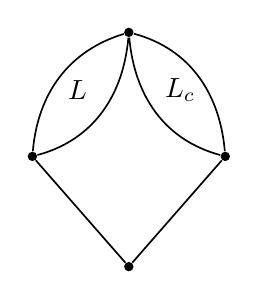
\begin{tikzpicture}[scale=0.7]
  \node (G) at (0,6.25) [fill,circle,inner sep=1.2pt] {};
  \node (K1) at (-1.75,4) [fill,circle,inner sep=1.2pt] {};
  \node (K2) at (1.75,4) [fill,circle,inner sep=1.2pt] {};
  \node (H) at (0,2) [fill,circle,inner sep=1.2pt] {};

\draw (-.93,5.2) node {$L$};
\draw (.93,5.2) node {$L_c$};


\draw[semithick] 
   (K1) to (H) to (K2)
   (G) to [out=197,in=85] (K1) 
   (K1) to [out=15,in=-95] (G)
   (G) to [out=-15,in=95] (K2) 
   (K2) to [out=165,in=-85] (G);

\end{tikzpicture}
\caption{}
\label{fig:twopanelchute}  
\end{figure}
As the next result shows, however, if a group property and its
negation are interval enforceable by the lattices $L$ and $L_c$, then already
at least one of these lattices is not group representable.
\begin{lemma}
\label{lemma:ie-prop-and-neg}
  If $\cP$ is a group property that is interval enforceable by a group representable lattice,
  then $\neg \cP$ is not interval enforceable by a group representable lattice.
\end{lemma}
\begin{proof}
Assume the contrary.  Then both $\cP$ and its negation $\neg \cP$
are interval enforceable by group representable lattices $L$ and $L_c$,
respectively. Let $G$ and $G_c$ be groups for which $L\cong [H,G]$ and $L_c\cong
[H_c,G_c]$ for some $H\leq G$ and $H_c\leq G_c$.
Then the group $G\times G_c$ has upper intervals 
$L\cong [H\times G_c, G\times G_c]$ and 
$L_c\cong [G\times H_c, G\times G_c]$.  Thus, by the interval enforceability
assumptions, the group $G\times G_c$ both is and is not a $\sG_\cP$-group. 
\end{proof}
To take a concrete example, insolubility is \IE.  However, solubility is
obviously not \IE. For, if $L\cong [H, G]$ then for any insoluble 
group $K$ we have $L\cong [H\times K, G\times K]$, and of course $G\times K$ is
insoluble.  Note that here (and in the proof 
of Lemma~\ref{lemma:ie-prop-and-neg}) the group $H\times K$ at the bottom of
the interval is not core-free.  So a more interesting question is whether a
property and its negation can both be cf-\IE.  Again, if such a property were
found, a lattice of the form in Figure~\ref{fig:twopanelchute} would give a
negative answer to the \FLRP, though this requires additional justification to address
the core-free aspect (see Section \ref{sec:parachute-lattices}).  
We suspect the answer is no, as suggested by
\begin{conjecture}
\label{conjecture:isle-prop2}
If $\cP$ is core-free interval enforceable by a group representable lattice,
then $\neg \cP$ is not core-free interval enforceable by a group representable lattice.
\end{conjecture}

We confirm a special case of the foregoing conjecture -- namely, the case when
$\cP$ is insolubility. Indeed, the following lemma implies that the class of
soluble groups, and more generally any class of groups that omits certain wreath
products, cannot be core-free interval enforceable by a group representable lattice.
\begin{lemma}
  \label{lem:IE-must-have-wreaths}
Suppose $\cP$ is core-free interval enforceable by a group
representable lattice.   
Then, for any finite nonabelian simple group $S$, there exists a wreath product group
of the form $W = S\wr \bar{U}$ that has property $\cP$.
\end{lemma}

\begin{proof}
  Let $L$ be a group representable lattice such that if $L\cong [H,G]$ and
  $\core_G(H)=1$ then $G\vDash \cP$.
  Since $L$ is group representable, there exists a $\cP$-group $G$ with $L
  \cong [H,G]$. 
  We apply an idea of Hans Kurzweil (see~\cite{Kurzweil:1985}) twice.
 %\footnote{A detailed description of Kurzweil's construction appears in~\cite[Section 2.2]{DeMeo:thesis}.} 
Fix a finite nonabelian simple
  group $S$. Suppose the index of $H$ in $G$ is $|G:H| = n$.
  Then the action of $G$ on the cosets of $H$ induces an automorphism of the
  group $S^n$ by permutation of coordinates.  Denote this representation by
  $\phi: G \rightarrow \Aut(S^n)$, 
  and let the image of $G$ be $\phi(G) =
  \bar{G} \leq \Aut(S^n)$.  
  The wreath product under this action is the group
  \[
  U:= S\wr_\phi G = S^n \rtimes_\phi G = S^n \rtimes \bar{G}, % =  S\wr \bar{G},
  \]
  with multiplication given by
  \[
  (s_1, \dots, s_n, x) (t_1, \dots, t_n, y) = 
  (s_1 t_{x(1)}, \dots, s_nt_{x(n)}, x y),
  \]
  for $s_i, t_i \in S$ and $x, y \in \bar{G}$.  (For the remainder of the proof,
  we suppress the semidirect product symbol and write, for example, $S^n\bar{G}$
  instead of $S^n \rtimes \bar{G}$.)

  An illustration of the subgroup lattice of such a wreath product appears in
  Figure~\ref{fig:kurzweil}.  Note that the interval
  $[D, S^n]$, where $D$ denotes the diagonal subgroup of
  $S^n$, is isomorphic to $\Eq(n)'$, the dual of the lattice of partitions of an
  $n$-element set.
  The dual lattice $L'$ is an upper interval of $\Sub(U)$, namely,
  $L'\cong [D\bar{G}, U]$.\footnote{These facts, which were proved by Kurzweil
    in~\cite{Kurzweil:1985}, are discuss in greater detail in~\cite[Section 2.2]{DeMeo:thesis}.} 

  \begin{figure}[!h]
\begin{center}
  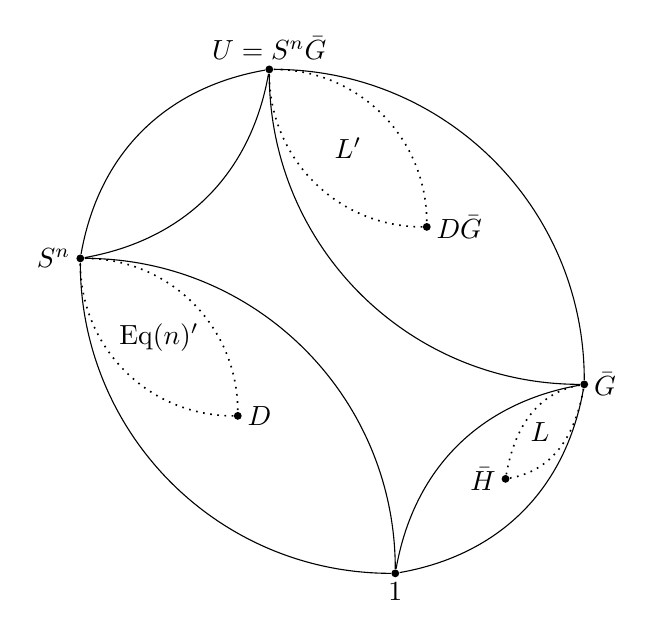
\begin{tikzpicture}[scale=.8]
    \node (G) at (3,3) [fill,circle,inner sep=1pt] {}; 
    \draw (G) node [right] {$\bar{G}$};
    \node (H) at (1.75,1.5) [fill,circle,inner sep=1pt] {}; 
    \draw (H) node [left] {$\bar{H}$};
    \node (Sn) at (-5,5) [fill,circle,inner sep=1pt] {}; 
    \draw (Sn) node [left] {$S^n$};
    \node (D) at (-2.5,2.5) [fill,circle,inner sep=1pt] {}; 
    \draw (D) node [right] {$D$};
    \node (DG) at (0.5,5.5) [fill,circle,inner sep=1pt] {}; 
    \draw (DG) node [right] {$D \bar{G}$};
    \node (1) at (0,0) [fill,circle,inner sep=1pt] {}; 
    \draw (1) node [below] {$1$};
    \node (SnG) at (-2,8) [fill,circle,inner sep=1pt] {}; 
    \draw (SnG) node [above] {$U=S^n \bar{G}$};
   \draw
    (G) to [out=190,in=80] (1) to [out=10,in=-100] (G)
    (Sn) to [out=0,in=90] (1) to [out=180,in=-90] (Sn)
    (SnG) to [out=190,in=80] (Sn) to [out=10,in=-100] (SnG)
    (SnG) to [out=0,in=90] (G) to [out=180,in=-90] (SnG);
    \draw[dotted, semithick]
    (G) to [out=190,in=80] (H) to [out=10,in=-100] (G)
    (SnG) to [out=0,in=90] (DG) to [out=180,in=-90] (SnG)
    (Sn) to [out=0,in=90] (D) to [out=180,in=-90] (Sn);
    \draw 
    (-3.75,3.75) node {$\Eq(n)'$}
    (-.75,6.75) node {$L'$}
    (2.3,2.25) node {$L$};
  \end{tikzpicture}
\end{center}
    \caption{Hasse diagram illustrating some features of the subgroup lattice of
      the wreath product $U$.}
%\caption{}
    \label{fig:kurzweil}
  \end{figure}
  It is important to note (and we prove below) that if $H$ is core-free in $G$ --
  equivalently, if $\ker \phi = 1$ -- then the foregoing construction results in
  the subgroup $D\bar{G}$ being core-free in $U$.  Therefore, by repeating the
  foregoing procedure, with  
  $H_1 = D\bar{G}$ denoting the (core-free) subgroup of $U$ such that $L' \cong
  [H_1, U]$, we find that $L = L''\cong [D_1 \bar{U}, S^m\bar{U}]$, where $m = |U:H_1|$, and $D_1$ denotes the diagonal subgroup of $S^m$.
    Since $D_1\bar{U}$ will be core-free in $S^m \bar{U}$ %(as proved below), 
    then, it follows by the original hypothesis that $S^m \bar{U} = S \wr
    \bar{U}$ must have property $\cP$.

  To complete the proof, we check that starting with a core-free subgroup
  $H \leq G$ in the Kurzweil construction just described results in a
  core-free subgroup $D \bar{G} \leq U$.   Let $N = \core_U(D\bar{G})$.  Then, for all $w=(d,\dots, d, x) \in N$ and for all 
  $u = (t_1,\dots, t_n, g)\in U$, we have $u w u^{-1}\in N$. 
  Fix $w=(d,\dots, d, x) \in N$.  We will choose $u\in U$ so that
  the condition $u w u^{-1}\in N$ implies $x$ acts trivially on $\{1, \dots, n\}$.
  First note that if $u = (t_1,\dots, t_n, 1)$, then
  %ll other $t_k$ distinct, and $g=1$.  
  \begin{align*}
  u n u^{-1} &= (t_1,\dots, t_n, 1) (d, \dots, d, x) (t_1^{-1},\dots, t_n^{-1}, 1)\\
  &=(t_1 d \,t_{x(1)}^{-1},\dots, t_nd \,t_{x(n)}^{-1}, 1) \in N,
  \end{align*}
  and this implies that $t_1 d\, t_{x(1)}^{-1} = t_2 d\, t_{x(2)}^{-1} =\cdots = t_nd \,t_{x(n)}^{-1}$. 
  Suppose by way of contradiction that $x(1) = j\neq 1$.  Then, since $x$ is a
  permutation (hence, one-to-one), $x(k) \neq j$ for
  each $k\in \{2, 3, \dots, n\}$.  Pick one such $k$ other than $j$.
  (This is possible since $n = |G:H|>2$; for otherwise $H\subnormal G$
  contradicting $\core_G(H)=1$.) 
  Since $u \in U$ is arbitrary, we may assume
  $t_1 = t_k$ and $t_{x(1)}=t_j\neq t_{x(k)}$.  
  But this contradicts $t_1 d\, t_{x(1)}^{-1} = t_k d\, t_{x(k)}^{-1}$.
  Therefore, $x(1) = 1$.  The same argument shows that 
  $x(i) = i$ for each $1\leq i\leq n$, 
  and we see that
  $w=(d,\dots,d, x) \in N$ implies $x\in \ker \phi = 1$.  This puts $N$ below
  $D$, and the only normal subgroup of $U$ that lies 
  below $D$ is the trivial group.
\end{proof}
By the foregoing result we conclude that a class of groups that does
not include wreath products of the form $S\wr G$, where $S$ is an arbitrary
finite nonabelian simple group, is not a core-free interval enforceable class. 
The class of soluble groups is an example.

%\vskip2mm



\subsection{Dedekind's rule and its consequences}
\label{sec:dedekinds-rule}
When $A$ and $B$ are subgroups of a group $G$, by $AB$ we mean the set
$\{ a b \mid a\in A, b\in B\}$, and we write $A \join B$ or $\<A, B\>$ to denote
the subgroup of $G$ generated by $A$ and $B$.  
Clearly $AB \subseteq \<A,B\>$; 
equality holds if and only if $A$ and $B$ \emph{permute}, by which we mean $A B = B A$.

We will need the following standard theorem:\footnote{See, for example, page~122
  of Rose, \emph{A Course on Group Theory}~\cite{Rose:1978}.} 
\begin{theorem}[Dedekind's rule]
  \label{lemma-dedekind}
Let $G$ be a group and let $A, B$ and $C$ be subgroups of $G$ with $A\leq B$.  Then,
\begin{align}
\label{eq:dedekind1}
A(C\cap B) &= AC \cap B,\qquad \text{ and }\\
\label{eq:dedekind2}
(C\cap B)A &= CA \cap B.
\end{align}
\end{theorem}

Our next lemma (Lemma~\ref{lemma-wjd-4}) generalizes a standard
result.  We find this generalization useful for proving that certain properties are
core-free interval enforceable.
To state Lemma~\ref{lemma-wjd-4}, we need some new notation.  
Let $U$ and $H$ be subgroups of a group,
let $U_0 = U\cap H$, and consider the interval $[U_0, U]=\{ V \mid U_0 \leq V
\leq U\}$.   
It will be helpful to visualize part of the subgroup lattice of
$\<U,H\>$, as shown in Figure~\ref{fig:intervals}.


\begin{figure}[!h]
\begin{center}
%{\scalefont{.8}
  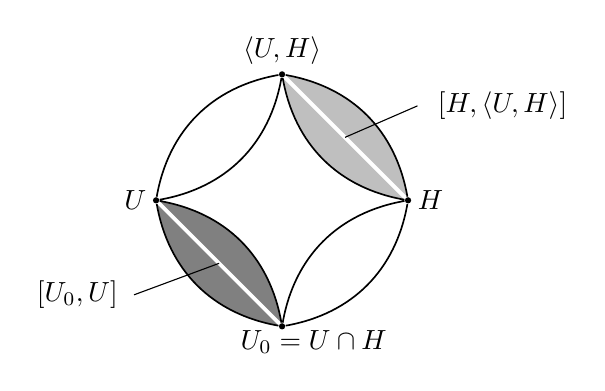
\begin{tikzpicture}[scale=.4]
    \node (H) at (4,4) [fill,circle,inner sep=\dotsize] {}; \draw (H) node [right] {$H$};
    \node (U) at (-4,4) [fill,circle,inner sep=\dotsize] {}; \draw (U) node [left] {$U$};
    \node (U0) at (0,0) [fill,circle,inner sep=\dotsize] {}; 
    \draw (1,-.5) node {$U_0 = U\cap H$};
    \node (UH) at (0,8) [fill,circle,inner sep=\dotsize] {}; \draw (UH) node
          [above] {$\<U,H\>$};
      \fill[color=gray] 
    (U) to [out=-10,in=100] (U0) to [out=170,in=-80] (U);
      \fill[color=lightgray] 
    (UH) to [out=-10,in=100] (H) to [out=170,in=-80] (UH);
   \draw[semithick]
     (H) to [out=190,in=80] (U0) to [out=10,in=-100] (H)
    (UH) to [out=190,in=80] (U) to [out=10,in=-100] (UH)
    (U) to [out=-10,in=100] (U0) to [out=170,in=-80] (U)
    (UH) to [out=-10,in=100] (H) to [out=170,in=-80] (UH);
    \draw (-6.5,1) node {$[U_0, U]$};
    \draw(-4.7,1) to (-2,2);
%     (-4,1) to [out=30,in=-90] (-2,2);

    \draw (7,7) node {$[H, \<U,H\>]$};
    \draw(4.3,7) to (2,6);

  \end{tikzpicture}
%}
\end{center}
  \caption{Some intervals in a subgroup lattice.}
  \label{fig:intervals}
\end{figure}

Recall that the usual isomorphism theorem for groups implies
that 
if $H$ is a normal subgroup of $\<U, H\>$, 
then the interval
$[H, \<U, H\>]$ is isomorphic to the interval $[U\cap H, U]$.  The 
purpose of the next lemma is to relate these two
intervals in cases where we drop the assumption $H\subnormal \<U,H\>$
and add the assumption $UH = \<U,H\>$.

If the two subgroups $U$ and $H$ permute, then we define 
\begin{equation}
  \label{eq:dedekind-1}
[U_0, U]^H = \{ V\in [U_0,U] \mid VH = HV\},
\end{equation}
which consists of those subgroups in $[U_0, U]$ that permute with
$H$. 

If $H$ normalizes $U$ (which implies $UH=HU$), 
then we % and in this case we  (in which case $UH$ is again be a group),
define
\begin{equation}
  \label{eq:dedekind-2}
[U_0, U]_H = \{ V\in [U_0,U] \mid H\leq N_{UH}(V)\}.
\end{equation}
This is the set consisting of those subgroups in $[U_0, U]$ that
are normalized by $H$ (sometimes called 
\emph{$H$-invariant subgroups} in $[U_0,U]$).
Notice that to even
define $[U_0, U]_H$ we must have $H\leq N_{UH}(U)$, and in this case, as we will
see below, the sublattices 
$[U_0, U]_H$ and $[U_0, U]^H$ coincide.

We are now ready to state the main result relating the sets defined
in~(\ref{eq:dedekind-1}) and (\ref{eq:dedekind-2}) %(when they exist) 
to the interval $[H, UH]$.
\begin{lemma}
  \label{lemma-wjd-4}
Suppose $U$ and $H$ are permuting subgroups of a group. %, that is, suppose $UH$ is a group.
Let $U_0 = U\cap H$.  Then
\begin{enumerate}[(i)]
\item $[H, UH]  \cong  [U_0, U]^H \leq [U_0, U]$.
\item If $U \subnormal UH$, then  $[U_0, U]_H  = [U_0, U]^H \leq [U_0, U]$.
\item If $H \subnormal UH$,  then  $[U_0, U]_H  = [U_0, U]^H = [U_0, U]$.
\end{enumerate}
\end{lemma}
\begin{remarks}
Part (ii) of Lemma~\ref{lemma-wjd-4} is a standard result (see, e.g.,
\cite{Borner:1999}). It seems likely that part (i) of the lemma is also well
known, though we have not seen it elsewhere. 
Since $G=UH$ is a group, the hypothesis of (ii) is equivalent to
$H\leq N_G(U)$, and the hypothesis of (iii) is equivalent to $U\leq N_G(H)$.
Part (i) of the lemma says that when two subgroups permute, we can
identify the interval above either one of them with the sublattice of
subgroups below the other that permute with the first.
Part (ii) is similar except we identify the interval above $H$ with
the  sublattice of $H$-invariant subgroups below $U$.  Once we have proved (i), the
proof of (iii) follows trivially from the standard isomorphism theorem for
groups, so we omit the details.
\end{remarks}

\begin{proof}
To prove (i), we first show that the following maps are inverse order isomorphisms:
\begin{align}
\label{eq:inverse-isos}
\phi: \;& [H, UH] \ni X \mapsto U\cap X \in [U_0, U]^H\\
\psi: \;& [U_0, U]^H \ni V \mapsto VH \in [H, UH].\nonumber
\end{align}
Then we show that $[U_0, U]^H$ is a sublattice of $[U_0,U]$, that is, 
$[U_0, U]^H\leq [U_0,U]$.

Fix $X\in [H, UH]$. We claim that $U\cap X \in [U_0, U]^H$. Indeed,
\[
    (U\cap X) H = UH \cap X=
               HU \cap X
                = H(U \cap X).
\]
The first equality holds by~(\ref{eq:dedekind2}) since $H\leq X$, the second holds
by assumption, and the third by~(\ref{eq:dedekind1}).
  This proves $U\cap X \in [U_0, U]^H$.  Moreover, by the first equality,
$\psi \circ \phi (X) = (U\cap X)H =UH \cap X = X$,
so $\psi \circ \phi$ is the identity on $[H, UH]$.

If $V\in [U_0, U]^H$, then $VH = HV$ implies $VH \in [H, UH]$. Also, $\phi \circ
\psi$ is the identity on $[U_0, U]^H$, since $\phi \circ \psi(V)= VH \cap U =
V(H\cap U)= VU_0 = V$, by~(\ref{eq:dedekind1}). 
This proves that $\phi$ and $\psi$ are inverses of each other on the sets indicated, and
it's easy to see that they are order preserving:
$X\leq Y$ implies $U\cap X \leq U\cap Y$, and $V\leq W$ implies $VH \leq WH$.
Therefore, $\phi$ and $\psi$ are inverse order isomorphisms.

To complete the proof of (i), we show that
$[U_0, U]^H$ is a sublattice of $[U_0, U]$.  Suppose $V_1$ and $V_2$ are
subgroups in $[U_0, U]$ that permute with $H$.  
It is easy to see that their join $V_1 \join V_2 = \<V_1, V_2\>$ also permutes
with $H$, so we just check that their intersection permutes with $H$.  Fix
$x \in V_1 \cap V_2$ and $h\in H$.  We show $xh = h'x'$ for some $h'\in H, \, x'
\in V_1\cap V_2$. Since $V_1$ and $V_2$ permute with $H$, we have $xh = h_1 v_1$
and $xh = h_2 v_2$ for some $h_1, h_2\in H, \, v_1 \in V_1, \, v_2 \in V_2$.
Therefore, $h_1 v_1 = h_2 v_2$, which implies $v_1 = h_1^{-1}h_2 v_2 \in HV_2$,
so $v_1$ belongs to $V_1 \cap HV_2$. Note that $V_1 \cap HV_2$ is below both $V_1$ and
$U\cap HV_2 = \phi \psi(V_2) = V_2$.  Therefore, $v_1 \in V_1 \cap HV_2 \leq V_1
\cap V_2$, and we have proved that $xh = h_1 v_1$ for $h_1\in H$ and $v_1 \in
V_1\cap V_2$, as desired. 

To prove (ii), assuming $U\subnormal G:=UH$, we show that if $U_0 \leq V \leq U$,
then $VH = HV$ if and only if $H\leq N_G(V)$.
If $H\leq N_G(V)$, then $VH = HV$ (even when $U \notsubnormal G$).
Suppose $VH = HV$.  We must show $(\forall v\in V)\, (\forall h\in H)\; hvh^{-1}\in
V$.  Fix $v\in V, \, h\in H$.  Then, $hv = v'h'$ for some $v'\in V,\, h'\in H$, since
$VH = HV$.  Therefore, $v' h' h^{-1} = hvh^{-1} = u$ for some $u\in U$, since
$H\leq N_G(U)$. This proves that $hvh^{-1}\in VH\cap U = V(H\cap U) = VU_0 = V$, as
desired.
\end{proof}

\subsection{Parachute lattices}
\label{sec:parachute-lattices}
We now prove the equivalence of statements (B), (C), 
and (D) mentioned in Section~\ref{sec:intro}.  
(That statement (E) of Section~\ref{sec:intro} is also equivalent to (B) follows
easily from the arguments given below, so we omit the details.)
\begin{theorem}
\label{thm-wjd-1}
The following statements are equivalent:
\begin{enumerate}
\item[(B)] Every finite lattice is isomorphic to
  an interval in the subgroup lattice of a finite group.
\item[(C)]
For every finite lattice $L$, for every finite collection $\sG_1, \dots, \sG_n$
of cf-\IE\ classes of groups,
there exists a finite group $G \in \bigcap\limits_{i=1}^n \sG_i$ such that $L \cong
[H,G]$ for some core-free subgroup $H\leq G$. % core-free in $G$.
%$\core_G(H) = 1$.

\item[(D)]
For every finite collection $\sL$ of finite lattices, there exists a finite
group $G$ such that each $L_i \in \sL$ is isomorphic to $[H_i, G]$ for some
core-free subgroup $H_i\leq G$.

\item[(E)]
For every finite collection $\sL$ of finite lattices, for every finite collection $\sG_1, \dots, \sG_n$
of cf-\IE\ classes of groups,
there exists a finite group $G \in \bigcap\limits_{i=1}^n \sG_i$ such that for
each $L_i \in \sL$ we have $L_i\cong [H_i, G]$ for some subgroup
$H_i$ that is core-free in $G$. % for some core-free $H_i\leq G$. 
\end{enumerate}
\end{theorem}
\begin{remark}
By (C), the \FLRP\ would have a negative answer if we
could find a collection $\sG_1, \dots, \sG_n$ of cf-\IE\ classes
such that $\bigcap\limits_{i=1}^n \sG_i$ is empty.
\end{remark}

\begin{proof}
We prove the equivalence of (B) and (C). 
Obviously (C) implies (B).  Assume (B) holds and let $L$ be any finite lattice.  Suppose 
$\sG_1, \dots, \sG_n$ is a collection of cf-\IE\ enforceable classes of groups.
Then there exist finite lattices $L_1, \dots, L_n$ such that $L_i \cong [H_i, G_i]$
with $\core_G(H_i)=1$ implies $G_i\in \sG_i$.
Construct a new lattice, denoted $\sP = \sP(L, L_1, \dots, L_n)$, as shown in
the Hasse diagram of Figure~\ref{fig:parachute} (a).  Note that the bottoms of
the $L_i$ sublattices are atoms in $\sP$.
\begin{figure}[centering]
  \caption{The parachute construction.}
  \label{fig:parachute}
\begin{center}
{\scalefont{.8}
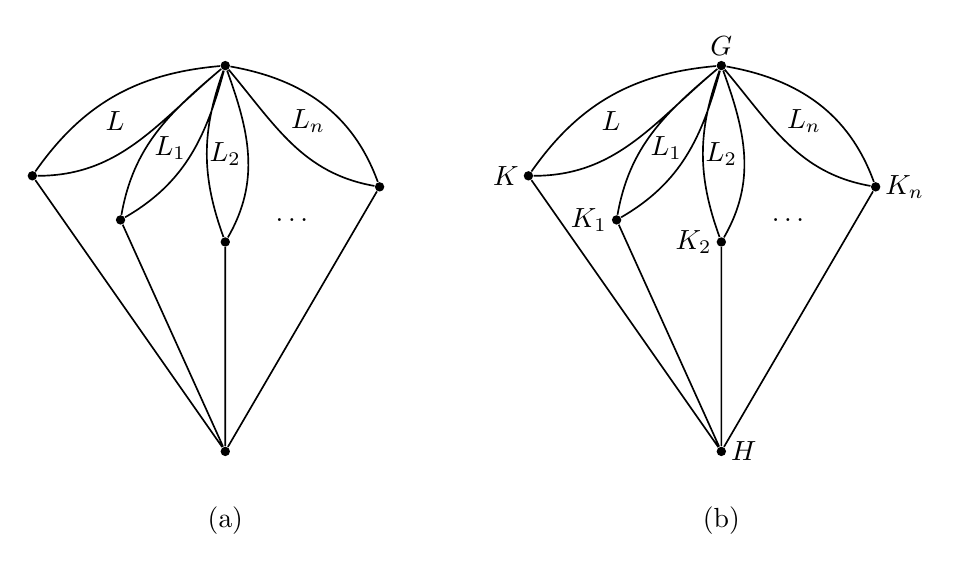
\begin{tikzpicture}[scale=0.7]

  \node (G) at (-8,0) [fill,circle,inner sep=1.2pt] {};
  \node (K) at (-11.5,-2) [fill,circle,inner sep=1.2pt] {};
  \node (K1) at (-9.9,-2.8) [fill,circle,inner sep=1.2pt] {};
  \node (K2) at (-8,-3.2) [fill,circle,inner sep=1.2pt] {};
  \node (Kn) at (-5.2,-2.2) [fill,circle,inner sep=1.2pt] {};
  \node (H) at (-8,-7) [fill,circle,inner sep=1.2pt] {};

\draw (-10,-1) node {$L$};
\draw (-9,-1.5) node {$L_1$};
\draw (-8,-1.6) node {$L_2$};
\draw (-6.5,-1) node {$L_n$};
\draw (-6.75,-2.8) node {$\dots$};

\draw (-8,-8.25) node {(a)};

\draw[semithick] 
   (K) to (H) to (K1)
   (K2) to (H) to (Kn);

\draw [semithick]  
   (G) to [out=-140,in=0] (K)
   (K)  to [out=55,in=185] (G)
   (G) to [out=-105,in=30] (K1)
   (K1) to [out=80,in=-140] (G)
   (G) to [out=-70,in=60] (K2)
   (K2)  to [out=110,in=-110] (G)
   (G) to [out=-10,in=110] (Kn)
   (Kn)  to [out=170,in=-50] (G);

%%% second (labelled) parachute %%%

  \node (Gr) at (1,0) [fill,circle,inner sep=1.2pt] {};
  \node (Kr) at (-2.5,-2) [fill,circle,inner sep=1.2pt] {};
  \node (K1r) at (-0.9,-2.8) [fill,circle,inner sep=1.2pt] {};
  \node (K2r) at (1,-3.2) [fill,circle,inner sep=1.2pt] {};
  \node (Knr) at (3.8,-2.2) [fill,circle,inner sep=1.2pt] {};
  \node (Hr) at (1,-7) [fill,circle,inner sep=1.2pt] {};

\draw (-1,-1) node {$L$};
\draw (0,-1.5) node {$L_1$};
\draw (1,-1.6) node {$L_2$};
\draw (2.5,-1) node {$L_n$};
\draw (2.25,-2.8) node {$\dots$};
\draw (1,-8.25) node {(b)};


\draw (Gr) node [above] {$G$}
    (Kr) node [left] {$K$}
    (K1r) node [left] {$K_1$}
    (K2r) node [left] {$K_2$}
    (Knr) node [right] {$K_n$}
    (Hr) node [right] {$H$};

\draw[semithick] 
   (Kr) to (Hr) to (K1r)
   (K2r) to (Hr) to (Knr);

\draw [semithick]  
   (Gr) to [out=-140,in=0] (Kr)
   (Kr)  to [out=55,in=185] (Gr)
   (Gr) to [out=-105,in=30] (K1r)
   (K1r) to [out=80,in=-140] (Gr)
   (Gr) to [out=-70,in=60] (K2r)
   (K2r)  to [out=110,in=-110] (Gr)
   (Gr) to [out=-10,in=110] (Knr)
   (Knr)  to [out=170,in=-50] (Gr);
\end{tikzpicture}
}
\end{center}
\end{figure}
By (B), there exist groups $H <G$ with $\sP \cong [H,G]$.  We can assume $H$
is a core-free subgroup of $G$.  (If not, replace $G$ and $H$ with
$G/N$ and $H/N$, where $N=\core_G(H)$, and note that 
$\sP \cong [H,G] \cong [H/N,G/N]$.)
Let $K, K_1, \dots, K_n$ be the subgroups of $G$ in which $H$ is maximal
and for which
$L \cong [K, G]$ and $L_i \cong [K_i, G],\; 1\leq i\leq n$ (Figure~\ref{fig:parachute} (b)).
If we can prove for each $1\leq i\leq n$ that $\core_G(K_i)=1$, then $G\in
\sG_i$ by hypothesis, and it will follow that $G \in \bigcap\limits_{i=1}^n
\sG_i$, proving that (B) implies (C). 

If $L \cong \2$, the two element lattice, or if $L_j\cong \2$ for all $1\leq
j\leq n$, then the theorem is vacuously true.  So we can assume without loss of
generality that $L\ncong \2$ and that there is at least one $1\leq j\leq n$ for which
$L_j\ncong \2$. Let $N$ be a minimal normal subgroup of $G$ and suppose $N\leq
K_i$.  Since $H$ is core-free, $K_i = NH$.  
Suppose $K_i \neq K$.
Note that the groups $K$ and $K_i$ permute:
\[
K K_i = K NH = NKH = NHK = K_i K.
\]
Therefore, by Lemma~\ref{lemma-wjd-4} (i) we see that the interval $[K,G] \cong L$
must be isomorphic to a sublattice of the interval $[H,K_i]\cong \2$, but this
contradicts $L\ncong \2$.
Suppose instead that $K = K_i$. Note that $K \neq K_j$, and since $K=NH$, we
see that $K$ and $K_j$ permute.  Therefore, by Lemma~\ref{lemma-wjd-4} (i)
again, the lattice $L_j\ncong \2$ is isomorphic to a sublattice of $[H,K]\cong
\2$, which is impossible.  This proves that $NH = G$ for all $N\subnormal G$, so
each $K_i$ is core-free. 

The proof that statements (B) and (D) are equivalent follows by a similar
construction.  Roughly, if
$\sL = \{L_1, \dots, L_n\}$, we form  the lattice $\sP = \sP(L_1, \dots, L_n)$.
If (B) holds, then there exists a group $G$ with $\sP \cong [H, G]$ and
$\core_G(H)=1$.  The proof that each $K_i$ is core-free, where $L_i\cong [K_i,G]$, is
similar to the argument above.
\end{proof}

By a \emph{parachute lattice}, denoted $\sP(L_1, \dots, L_m)$,
we mean a lattice just like the one illustrated in 
Figure~\ref{fig:parachute} (a), but with the lattices $L_1, \dots, L_m$
appearing as the upper intervals. %, and the bottom of each $L_i$ covering the bottom of $\sP(L_1, \dots, L_m)$.

Next we prove that %Lemma~\ref{lemma-wjd-5} says that 
any group that has a nontrivial parachute lattice as an upper interval
in its subgroup lattice must have some rather special properties.  
\begin{lemma}
\label{lemma-wjd-5}
 Let $\sP = \sP(L_1, \dots, L_n)$ with $n\geq 2$ and $|L_i|>2$ for all
%\; (1\leq i\leq n)$, 
$i$, and suppose $\sP \cong [H, G]$, with $H$ core-free in $G$.  
\begin{enumerate}[(i)]
\item If $1\neq N \subnormal G$, then $NH = G$ and $C_G(N)=1$.
\item $G$ is subdirectly irreducible and insoluble.
\end{enumerate}
\end{lemma}
\begin{remark}
If a subgroup $N\leq G$ is abelian, then $N \leq C_G(N)$, so (i) implies
that every nontrivial normal subgroup of $G$ is nonabelian.  
\end{remark}
\begin{proof}
(i)
Let $1\neq N \subnormal G$.  Then $N \nleq H$, since $H$ is core-free in $G$.
Therefore, $H < NH$.   As in Section \ref{sec:parachute-lattices}, we let $K_i$
denote the subgroups of $G$ 
corresponding to the atoms of $\sP$.  
Then $H$ is covered by each $K_i$, so $K_j\leq NH$ for some $1\leq j\leq n$.  
Suppose, by way of contradiction, that $NH < G$.  
By assumption, $n\geq 2$ and $|L_i|>2$.  Thus for any $i\neq j$ we have
$K_i\leq Y < Z < G$ for some subgroups $Y$ and $Z$ which satisfy
$(NH)\cap Z = H$ and $(NH)\join Y = G$.  Also, $(NH)Y = NY$ is a group, so
$(NH)Y=NH\join Y = G$.  But then, by Dedekind's rule, we have
\[
Y = HY = ((NH)\cap Z) Y = (NH)Y \cap Z = G\cap Z = Z,
\]
contrary to $Y<Z$.  This contradiction proves that $NH = G$.

To prove that $C_G(N)=1$, let $M$ be a minimal normal subgroup of $G$
contained in $N$.  It suffices to prove $C_G(M)= 1$.
Assume the contrary. Then, 
since $C_G(M) \subnormal N_G(M) =G$, it follows by
what we just proved that $C_G(M)H = G$.
Consider any $H< K < G$. Then $1 < M\cap K < M$ (strictly, by
Lemma~\ref{lemma-wjd-4}). Now $M\cap K$ is normalized by $H$ and centralized
(hence normalized) by $C_G(M)$.  
%(Indeed, $C_G(M)$ centralizes every subgroup of $M$.) 
Therefore, $M\cap K \subnormal C_G(M)H = G$, contradicting the minimality of
$M$.  

To prove (ii) we first show that $G$ has a unique minimal normal subgroup.  Let
$M$ be a minimal
%\footnote{If $G$ is simple, then $M = G$; ``minimal'' assumes nontrivial.} 
normal subgroup of $G$ and let $N \subnormal G$ be any normal subgroup not 
containing $M$.  We show that $N = 1$.  Since both subgroups
are normal, the commutator subgroup
$[M,N]$
lies in the intersection $M\cap N$, which is trivial by the minimality of $M$.   
Thus, $M$ and $N$ centralize each other.  In particular,
$N \leq C_G(M) = 1$, by (i).

Finally, since $G$ has a unique
minimal normal subgroup that is nonabelian 
(see the remark preceding the proof),
$G$ is insoluble.
\end{proof}

To summarize what we have thus far, the lemmas above imply that (B) holds if and only if
every finite lattice is an interval $[H, G]$, with $H$ core-free in $G$, where
\begin{enumerate}[(i)]
\item $G$ is insoluble, not alternating, and not symmetric;
\item $G$ has a unique minimal normal subgroup $M$ which satisfies $MH = G$
and $C_G(M) = 1$; in particular,
$M$ is nonabelian and $\core_G(X) = 1$ for all $H\leq X < G$.
\end{enumerate}

Finally, we recall that the structure of the unique minimal normal subgroup can be
described as follows (see, e.g., \cite[Theorem 4.3.A]{Dixon:1996}):
\begin{enumerate}[(i)]
\item[(iii)] $M = T_0\times \cdots \times T_{r-1}$, where $T_i$ are simple minimal normal subgroups of
  $M$ which are conjugate (under conjugation by elements of $G$). Thus, $M$ is a
  direct power of a simple group $T$.
\end{enumerate}
  In fact, when $C_G(M)=1$, as in our application,
we can specify these conjugates more precisely. % in terms of elements of $H$.
Let $T$ be any minimal normal subgroup of $M$. Note that $T$ is simple.
Let $N = N_H(T) = \{h\in H : T^h = T\}$ be the normalizer of $T$ in
$H$.  Then the proof of the following lemma is routine, so we omit it.
\begin{lemma}
If $H/N = \{N, h_1N, \dots, h_{k-1}N\}$ is a full set of left cosets of $N$
in $H$, then $k=r$ and $M = T_0\times \cdots \times T_{r-1} = T \times
T^{h_1} \times T^{h_{r-1}}$. 
\end{lemma}

We conclude this section by noting that other researchers, such as Baddeley,
B\"orner, and Lucchini, have proved similar results 
for a more general class of lattices called 
\defn{LP-lattices}.\footnote{An LP-lattice is one in which
  every element except $0$ and $1$ is a non-modular element.}
These authors observe that a group having an L-P lattice as an upper
interval in its subgroup lattice must be a \emph{quasiprimitive permutation group}. 
We remark that a parachute lattice in which each panel
 $L_i$ has $|L_i|>2$ is an LP-lattices, so
Lemma~\ref{lemma-wjd-5} follows from
theorems of Baddeley, B\"orner, Lucchini, et al. 
(cf.~\cite{Lucchini:1997}, \cite{Borner:1999}).
However, the main purpose of our construction is not only to
provide a quick route to Lemma~\ref{lemma-wjd-5}, but also to
demonstrate a natural way to insert arbitrary finite lattices
$L_i$ as upper intervals $[K_i, G]$ in $\Sub(G)$, with $K_i$ core-free in
$G$, so that once we establish a number of cf-\IE\ properties,
it will follow that \emph{every} finite lattice $L$ must be isomorphic to an upper
interval $L \cong [K, G]$ for some $G$ satisfying all of these cf-\IE\ properties,
if the \FLRP\ is to have a positive answer.   

We conclude this section by formalizing the remarks of the previous sentence.
Given two group theoretical properties $\cP_1, \cP_2$, we write
$\cP_1 \rightarrow \cP_2$ to denote that property 
$\cP_1$ implies property $\cP_2$. In other words,
$G\vDash \cP_1$ only if $G\vDash \cP_2$.
Thus $\rightarrow$ provides a natural partial order on any given set of 
properties, as follows:
\[
\cP_1 \leq \cP_2\quad  \Longleftrightarrow \quad \cP_1 \rightarrow \cP_2 \quad
\Longleftrightarrow \quad \sG_{\cP_1}\subseteq
\sG_{\cP_2},
\]
where $\sG_{\cP_i} = \{G\in \G \mid G\vDash \cP_i\}$.
The following is an immediate corollary of the parachute construction
described above.
\begin{corollary}
\label{cor:isle-prop-groups-1}
  If $\sP = \{\cP_i \mid i\in \sI\}$ is a collection of (cf-)\IE\ properties,
  then $\Meet \sP$ is (cf-)\IE.
\end{corollary}
The conjunction $\Meet \sP$ corresponds to the class 
$\bigcap_{i\in \sI} \sG_{\cP_i} = \{G \in \G \mid (\forall i \in \sI) \; G\vDash
\cP_i \}$.

\section{An application}
\label{sec:application}
We consider an application that 
demonstrates the utility of Lemma~\ref{lemma-wjd-4} for identifying certain core-free
interval enforceable properties.
The lattice that we study in this section 
has special relevance to the finite lattice representation problem (\FLRP).

In prior 
work,\footnote{Universal algebra and lattice theory seminar, University of
  Hawaii, 2010-11; participants: Ralph Freese, Tristan
  Holmes, Peter Jipsen, Bill Lampe, J.B.~Nation and the author.}
 we considered whether, for every
lattice $L$ with at most $n$ elements, there exists a finite algebra with a
congruence lattice that is isomorphic to $L$.
For $n=6$, the problem had already been solved.
In fact, Aschbacher~\cite{Aschbacher:2008} and Watatani~\cite{Watatani:1996}
prove that every lattice with at most 6 elements is group representable
(as defined in Section \ref{sec:negat-interv-enforc} above).  
For $n=7$, although we have not found them all as intervals in subgroup lattices, we have
found congruence lattice representations for all lattice with at most 7 elements
with one exception (see~\cite{overalgebras}, \cite{DeMeo:thesis}). 
The exceptional lattice, which we call $L_7$, appears in
Figure~\ref{fig:L7}. Thus $L_7$ is the smallest lattice for which we have not
found a representation of the form $L_7\cong \Con\bA$ for some finite algebra
$\bA$.

\begin{figure}[h!]
\begin{center}
  {\scalefont{.8}
    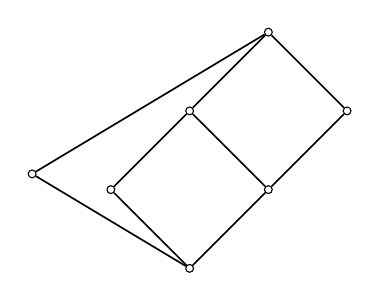
\begin{tikzpicture}[scale=1]
      \node (J1) at (0,1)  [draw, circle, inner sep=1pt] {};
      \node (H) at (1,0)  [draw, circle, inner sep=1pt] {};
      \node (M2) at (1,2)  [draw, circle, inner sep=1pt] {};
      \node (J2) at (2,1)  [draw, circle, inner sep=1pt] {};
      \node (G) at (2,3)  [draw, circle, inner sep=1pt] {};
      \node (M1) at (3,2)  [draw, circle, inner sep=1pt] {};
      \node (K) at (-1,1.2)  [draw, circle, inner sep=1pt] {};
      \draw[semithick] (H) to (J1) to (M2) to (G) to (M1) to (J2) to (H) (J2) to (M2);
      \draw[semithick] (H) to (K) to (G);
    \end{tikzpicture}
  }
\end{center}
  \caption{The exceptional seven element lattice, $L_7$.}
  \label{fig:L7}
\end{figure}

Suppose $\bA$ is a finite algebra with $\Con \bA \cong L_7$, and
suppose $\bA$ is of minimal cardinality among those algebras having
a congruence lattice isomorphic to $L_7$.  Then 
$\bA$ must be isomorphic to a transitive \Gset.
(This fact is proved in the forthcoming article~\cite{gsets}.)  
Therefore, if $L_7$ is representable, we can assume there is a finite group $G$ with a 
core-free
subgroup $H<G$ such that $L_7$ is isomorphic to the interval
sublattice $[H,G] \leq \Sub(G)$.  In this section we present some restrictions
on the possible groups for which this can occur.  

The first restriction, which is
the easiest to observe, is that $G$ must act primitively on the cosets of one of its
maximal subgroups.  This suggests the possibility of describing $G$ in terms of
the Aschbacher-O'Nan-Scott Theorem which characterizes primitive
permutation groups.\footnote{The author thanks John Shareshian for 
this suggestion. See the comments at MathOverflow~\cite{MO85724}.}
Ultimately, the goal would be to find enough
restrictions on $G$ so as to rule out all finite groups.  As yet, we have not
achieved this goal.  However, the new results in this section reduce the
possibilities to special subclasses of the Aschbacher-O'Nan-Scott
Theorem.  This paves the way for future studies to focus on these subclasses
when searching for a group representation of $L_7$, or proving that none exists.

\begin{prop}
\label{thm:except-seven-elem}
Suppose $G$ is a finite group with $[H,G]\cong L_7$ for some core-free subgroup $H<G$.  Then the following hold.
\begin{enumerate}[(i)]
\item $G$ is a primitive permutation group.
\item If $N\ssubnormal G$, then $C_G(N) = 1$.
\item $G$ contains no non-trivial abelian normal subgroup.
\item $G$ is insoluble.
\item $G$ is subdirectly irreducible.
\item With the possible exception of at most one maximal subgroup,
  all proper subgroups in the interval $[H,G]$ are core-free. 

\end{enumerate}
\end{prop}
\begin{remark}
  It is obvious that (ii) $\Rightarrow$ (iii) $\Rightarrow$ (iv), and  (ii) $\Rightarrow$
  (v), but we include these easy consequences in the statement of the result for
  emphasis; for, although the hard work will be in proving (ii) and (vi), our
  main goal is the pair of restrictions (iii) and (v), which allow us to rule
  out a number of the O'Nan-Scott types describing primitive permutation
  groups.  
\end{remark}

Assume the hypotheses of the proposition above.  In particular, throughout this
section \emph{all groups are finite, $H$ is a core-free subgroup of $G$, and $[H,G] \cong
  L_7$}. Label the seven subgroups of $G$ in
the interval $[H,G]$ as in the following diagram:

\begin{center}
  {\scalefont{.8}

    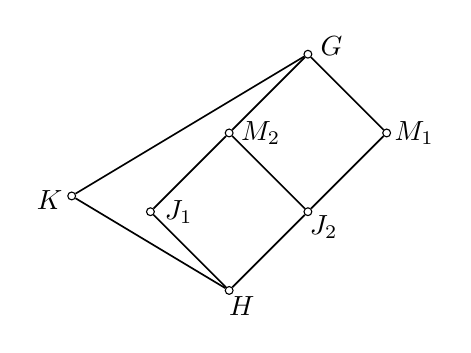
\begin{tikzpicture}[scale=1]
      \node (J1) at (0,1)  [draw, circle, inner sep=1pt] {};
      \draw (.36, 1) node {$J_1$};
      \node (H) at (1,0)  [draw, circle, inner sep=1pt] {};
      \draw (1.16, -.2) node {$H$};
      \node (M2) at (1,2)  [draw, circle, inner sep=1pt] {};
      \draw (1.4, 2) node {$M_2$};
      \node (J2) at (2,1)  [draw, circle, inner sep=1pt] {};
      \draw (2.2, .8) node {$J_2$};
      \node (G) at (2,3)  [draw, circle, inner sep=1pt] {};
      \draw (2.3, 3.1) node {$G$};
      \node (M1) at (3,2)  [draw, circle, inner sep=1pt] {};
      \draw (3.35, 2) node {$M_1$};
      \node (K) at (-1,1.2)  [draw, circle, inner sep=1pt] {};
      \draw (-1.28, 1.15) node {$K$};

      \draw[semithick] (H) to (J1) to (M2) to (G) to (M1) to (J2) to (H) (J2) to (M2);
      \draw[semithick] (H) to (K) to (G);

    \end{tikzpicture}
  }
\end{center}
% (The labels are chosen with the intention of helping us remember to which
% subgroups they refer:
% the maximal subgroup $M_2$ covers two subgroups in the interval
% $[H,G]$, while $J_2$ is covered by two subgroups of $G$.)

We now prove the foregoing proposition through a series of claims.
The first thing to notice about the interval $[H,G]$ is that
$K$ is a \defn{non-modular element} of the interval.  This means that
there is a pentagonal ($N_5$) sublattice of the interval with $K$ as the
incomparable proper element. (See the diagram below, for example.)
\begin{center}
  {\scalefont{.8}
    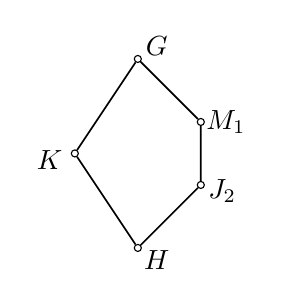
\begin{tikzpicture}[scale=.8]
      \node (H) at (0,0)  [draw, circle, inner sep=.9pt] {};
      \draw (.3, -.2) node {$H$};
      \node (K) at (-1,1.5)  [draw, circle, inner sep=.9pt] {};
      \draw (-1.4, 1.4) node {$K$};
      \node (11) at (1,1)  [draw, circle, inner sep=.9pt] {};
      \draw (1.34, .9) node {$J_2$};
      \node (12) at (1,2)  [draw, circle, inner sep=.9pt] {};
      \draw (1.4, 2) node {$M_1$};
      \node (G) at (0,3)  [draw, circle, inner sep=.9pt] {};
      \draw (.3, 3.2) node {$G$};
      \draw[semithick] (H) to (11) to (12) to (G) to (K) to (H);
    \end{tikzpicture}
}
\end{center}
Using this non-modularity property of $K,$ it is easy to 
prove the following
\begin{claim}
\label{claim:K1corefree}
$K$ is a core-free subgroup of $G$.
\end{claim}
\begin{proof}
  Let $N = \core_G(K)$.  If $N \leq X$ for some $X \in \{M_1, M_2, J_1, J_2\}$, 
then $N < X\cap K = H$, so $N = 1$ (since $H$ is core-free).  If
  $N\nleq X$ for all $X \in \{M_1, M_2, J_1, J_2\}$, then $NJ_2 = G$.  But then
Dedekind's rule leads to the following contradiction:
\[
J_2 \leq M_1 \; \Longrightarrow \; J_2 = J_2(N\cap M_1) = J_2 N \cap M_1 =
G\cap M_1 = M_1.
\]
Therefore, $N = 1$.
\end{proof}
Note that (i) of the proposition follows from Claim~\ref{claim:K1corefree}.  Since
$K$ is core-free, $G$ acts faithfully on the
cosets $G/K$ by right multiplication.  Since $K$ is a maximal subgroup, the
action is primitive.

The next claim is slightly harder than the previous one as it requires the
more general consequence of Dedekind's rule that we established above in
Lemma~\ref{lemma-wjd-4} (i). 
\begin{claim}
$J_1$ and $J_2$ are core-free subgroups of $G$.
\end{claim}
\begin{proof}
First note that if $N\subnormal G$ then the subgroup $NH$
permutes\footnote{Recall, for subgroups $X$ and $Y$ of a group $G$, we define
  the \emph{sets} $XY = \{xy\mid x\in X, y \in Y\}$, and
  $YX = \{yx\mid x\in X, y \in Y\}$, and 
we say that $X$ and $Y$ are \defn{permuting subgroups} (or that $X$ and $Y$
permute, or that $X$ permutes with $Y$)
 provided the two sets $XY$ and $YX$ coincide, in which case the set forms a group:
$XY = \<X,Y\> = YX$.}
with any subgroup
containing $H$.  To see this, let $H \leq X \leq G$ and note that
\[
  NHX = NX = XN= XHN = XNH,
\]
since $H \leq X$ and $N\subnormal G$.

Suppose $1\neq N\leq J_1$ for some $N \ssubnormal G$. Then $NH = J_1$, so $J_1$ and $K$ are
permuting subgroups.
Since $J_1K = G$ and $J_1\cap K = H$,
Lemma~\ref{lemma-wjd-4} yields
\[
[J_1, G] \cong [H, K]^{J_1} := \{X \in[H, K] \mid J_1X=XJ_1 \}.
\]
But this is impossible since $[H, K]^{J_1} \leq [H,  K] \cong \2$, while $[J_1, G]\cong \3$.
This proves that $\core_G(J_1) = 1$.
The intervals involved in the argument are drawn with bold lines in the
following diagram.
\begin{center}
  {\scalefont{.78}
   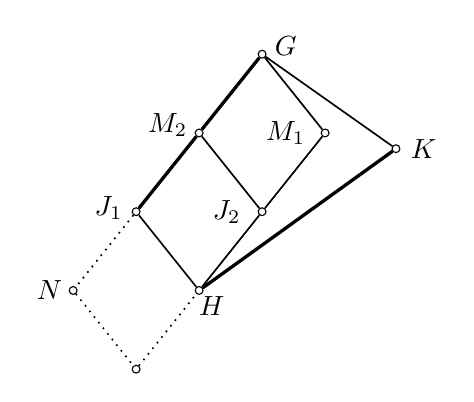
\begin{tikzpicture}[scale=1]
      \node (N) at (-.6,0)  [draw, circle, inner sep=1pt] {};
      \draw (-.9, 0) node {$N$};
      \node (NcapH) at (.2,-1)  [draw, circle, inner sep=1pt] {};
      \node (J1) at (0.2,1)  [draw, circle, inner sep=1pt] {};
      \draw (-.15, 1.05) node {$J_1$};
      \node (H) at (1,0)  [draw, circle, inner sep=1pt] {};
      \draw (1.16, -.2) node {$H$};
      \node (M2) at (1,2)  [draw, circle, inner sep=1pt] {};
      \draw (.6, 2.1) node {$M_2$};
      \node (J2) at (1.8,1)  [draw, circle, inner sep=1pt] {};
      \draw (1.35, 1.) node {$J_2$};
      \node (G) at (1.8,3)  [draw, circle, inner sep=1pt] {};
      \draw (2.1, 3.1) node {$G$};
      \node (M1) at (2.6,2)  [draw, circle, inner sep=1pt] {};
      \draw (2.1, 2) node {$M_1$};
      \node (K) at (3.5,1.8)  [draw, circle, inner sep=1pt] {};
      \draw (3.85, 1.8) node {$K$};
      \draw[semithick,dotted] (J1) to (N) to (NcapH) to (H);
      \draw[very thick] (J1) to (M2) to (G) (H) to (K);
      \draw[semithick] (H) to (J1) to (M2) to (G) to (M1) to (J2) to (H) to (K)
      to (G) (J2) to (M2);
    \end{tikzpicture}
 }
\end{center}

The proof 
that $J_2$ is core-free is similar.  Suppose
$1\neq N\leq J_2$ where $N \ssubnormal G$. Then $NH = J_2$ and the subgroups $J_2$ and $K$
permute.
Therefore, $[H, K]^{J_2} \cong [J_2, G]$, 
by Lemma~\ref{lemma-wjd-4},
which is a contradiction since
$[H, K]^{J_2} \leq [H,  K] \cong \2$, while $[J_2, G]\cong \two \times \two$.
\end{proof}

Now that we know $K, J_1, J_2$ are each core-free in $G$, we use this
information to prove that at least one of the other maximal subgroups, 
$M_1$ or $M_2$, is core-free in $G$, thereby establishing (vi) of the proposition.  
We will also see that $G$ is subdirectly irreducible, proving (v).  The proof of
(ii) will then follow from the same argument used to prove 
Lemma~\ref{lemma-wjd-4} (ii), which we repeat below.

\begin{claim}
  Either $M_1$ or $M_2$ is core-free in $G$.  If $M_2$ has non-trivial core
  and $N\ssubnormal G$ is contained in $M_2$, then
  $C_G(N)=1$ and $G$ is subdirectly irreducible.
\end{claim}
\begin{proof}
  Suppose $M_2$ has non-trivial core.  Then there is 
a minimal normal subgroup $1\neq N \ssubnormal G$ 
  contained in $M_2$. %, and therefore a minimal normal subgroup of $G$.  
  Since $H, J_1, J_2$ are core-free, $NH=M_2$.  Consider the centralizer,
  $C_G(N)$, of $N$ in $G$.  Of course, this is a normal subgroup 
  of $G$.\footnote{The centralizer of a normal subgroup $N\subnormal G$ is itself
    normal in $G$.  For, it is the kernel of the conjugation action of $G$ on
    $N$. Thus, $C_G(N) \subnormal N_G(N) = G$.} 
If $C_G(N) = 1$, then, since minimal normal subgroups
  centralize each other, $N$ must be the unique minimal normal subgroup of $G$.
  Furthermore, $M_1$ must be core-free in this case.  Otherwise 
  $N\leq M_1 \cap M_2 = J_2$, contradicting $\core_G(J_2)=1$. 
  Therefore, in case $C_G(N) = 1$ we 
  conclude that $G$ is subdirectly irreducible and $M_1$ is core-free.

  We now prove that the alternative, $C_G(N) \neq 1$, does not occur.
  This case is a bit more challenging and must be split up into further subcases,
  each of which leads to a contradiction.
  Throughout, the assumption $1\neq N \leq M_2$ is in force, and it helps to
  keep in mind the diagram in Figure~\ref{fig:M2-not-core-free}.
\begin{center}
  \begin{figure}
  {\scalefont{.8}
\begin{center}
   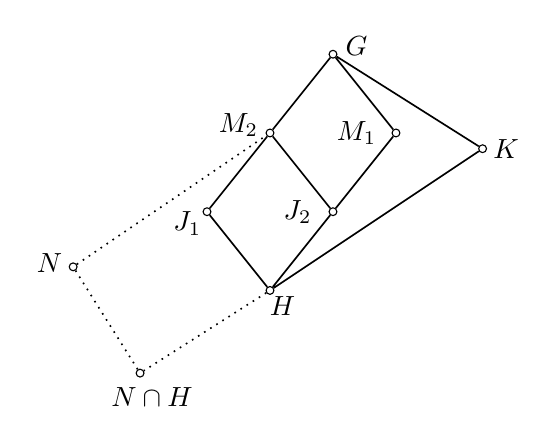
\begin{tikzpicture}[scale=1]
      \node (J1) at (0.2,1)  [draw, circle, inner sep=1pt] {};
      \draw (-.05, .85) node {$J_1$};
      \node (H) at (1,0)  [draw, circle, inner sep=1pt] {};
      \draw (1.16, -.2) node {$H$};
      \node (M2) at (1,2)  [draw, circle, inner sep=1pt] {};
      \draw (.6, 2.1) node {$M_2$};
      \node (J2) at (1.8,1)  [draw, circle, inner sep=1pt] {};
      \draw (1.35, 1.) node {$J_2$};
      \node (G) at (1.8,3)  [draw, circle, inner sep=1pt] {};
      \draw (2.1, 3.1) node {$G$};
      \node (M1) at (2.6,2)  [draw, circle, inner sep=1pt] {};
      \draw (2.1, 2) node {$M_1$};
      \node (K) at (3.7,1.8)  [draw, circle, inner sep=1pt] {};
      \draw (4, 1.8) node {$K$};
      \node (NcapH) at (-.65,-1.05)  [draw, circle, inner sep=1pt] {};
      \draw (-.5, -1.36) node {$N\cap H$};
      \node (N) at (-1.5,.3)  [draw, circle, inner sep=1pt] {};
      \draw (-1.8, .35) node {$N$};
      \draw[semithick, dotted]  (H) to (NcapH) (N) to (M2);
      \draw[semithick, dotted]
      (NcapH) to (N);
      \draw[semithick] 
      (H) to (J1) to (M2) to (G) to (M1) to (J2) to (H) to (K) to (G) 
      (J2) to (M2);
    \end{tikzpicture}
\end{center}
  }
    \caption{Hasse diagram illustrating the cases in which $M_2$ has
      non-trivial core: $1\neq N \leq M_2$ for some $N\ssubnormal G$.}
% \caption{}
    \label{fig:M2-not-core-free}
  \end{figure}
\end{center}

Suppose $C_G(N) \neq 1$.  Then, since $C_G(N)\subnormal G$,
and since $H, J_1, J_2, K$ are core-free, it's clear that $C_G(N)H \in
\{G, M_1, M_2\}$.  We consider each case separately.

\begin{enumerate}
\item[{\it Case 1:}] 
Suppose $C_G(N)H = G$.
Note that $N\cap H < N \cap J_1 < N$ (strictly). The
subgroup $N\cap J_1$ is normalized by $J_1$ and by $C_G(N)$, and so it is normal in
$C_G(N)J_1 \geq C_G(N)H = G$, contradicting the minimality of $N$.  Thus, the case
$C_G(N)H = G$ does not occur.

\item[{\it Case 2:}]
Suppose $C_G(N)H =M_1$.  The subgroup $N\cap J_1$ is
normalized by both $H$ and $C_G(N)$. For, $C_G(N)$ centralizes, hence
normalizes, every subgroup of $N$.  Therefore, $N\cap J_1$ is normalized by 
$C_G(N)H =M_1$.  Of course, it's also normalized by $J_1$, so
$N\cap J_1$ is normalized by the set $M_1J_1$, so it's normalized by the group
generated by that set, which is $\<M_1, J_1\> = G$.\footnote{Actually, the set is
already a group in this case since $M_1J_1 = C_G(N)H J_1 = J_1 C_G(N)H = J_1 M_1$.}
The conclusion is that $N\cap J_1\ssubnormal G$.  
Since $J_1$ is core-free, $N\cap J_1 = 1$.
But this contradicts the (by now familiar) consequence of
Dedekind's rule:  
\[
H < J_1 < M_2  \; \Longrightarrow \; N\cap H < N\cap J_1 < N\cap M_2.
\]
 Therefore, $C_G(N)H =M_1$ does not occur.

\item[{\it Case 3:}]
Suppose $C_G(N)H = M_2$.
The subgroup $N\cap M_1$ is
normalized by both $H$ and $C_G(N)$.  Therefore, $N\cap M_1$ is normalized by 
$C_G(N)H =M_2$.  Of course, it's also normalized by $M_1$, so
$N\cap M_1$ is normalized by $\<M_1, M_2\> = G$.
The conclusion is that $N\cap M_1\ssubnormal G$.  By 
minimality of the normal subgroup $N$, we must have either $N\cap M_1 = 1$ or 
$N\cap M_1 = N$.  The former equality implies $N\cap J_2=1$, which contradicts 
the strict inequalities of Dedekind's rule,
\begin{equation}
  \label{eq:6}
H < J_2 < M_2  \; \Longrightarrow \; N\cap H < N\cap J_2 < N\cap M_2,
\end{equation}
while the latter equality ($N\cap M_1 = N$) implies that $N \leq M_1 \cap M_2 = J_2$ which
contradicts 
$\core_G(J_2)=1$. 
\end{enumerate}
\end{proof}

We have proved that either $M_1$ or $M_2$ is core-free in $G$, and
we have shown that, if $M_2$ has non-trivial core, then $G$ is subdirectly
irreducible.  In fact, we proved that $C_G(N)=1$ for the unique minimal normal subgroup
$N$ in this case.  It remains to prove that $G$ is subdirectly irreducible in
case $M_1$ has non-trivial core. The argument is similar to the foregoing, and
we omit some of the details that can be checked exactly as above.

\begin{claim}
If $M_1$ has non-trivial core
  and $N\ssubnormal G$ is contained in $M_1$, then
  $C_G(N)=1$ and $G$ is subdirectly irreducible.
\end{claim}
\begin{proof}
If $M_1$ has non-trivial core, then there is a minimal normal
subgroup $N\ssubnormal G$ contained in $M_1$.  We proved above that
$M_2$ must be core-free in this case, so either $C_G(N)H  = G$, 
$C_G(N)H  = M_1$, 
or $C_G(N)=1$.  The first case is easily ruled out exactly as in Case 1 above. 
The second case is handled by the argument we used in Case 3.  Indeed, if we suppose 
$C_G(N)H = M_1$, 
then 
$N\cap M_2$ 
is normalized by both $H$ and $C_G(N)$, hence by
$M_1$.  It is also normalized by $M_2$, so 
$N\cap M_2\ssubnormal G$.  Thus, by minimality of $N$, 
and since $M_2$ is core-free,
$N\cap M_2 = 1$.  But then $N\cap J_2 = 1$,
leading to a contradiction similar to~(\ref{eq:6}) but with $M_1$ replacing $M_2$.  
Therefore, the case 
$C_G(N)H = M_1$ does not occur, and we have proved $C_G(N)=1$. 
\end{proof}


So far we have proved that all intermediate proper subgroups in the interval $[H, G]$
are core-free except possibly at most one of $M_1$ or $M_2$.  Moreover, we
proved that if one of the maximal subgroups has non-trivial core, then there is
a unique minimal normal subgroup $N\ssubnormal G$ with trivial centralizer,
$C_G(N) = 1$.  As explained above, $G$ is subdirectly irreducible in this case,
since minimal normal subgroups centralize each other.

In order to prove (ii), there remains only one case left to check, and the
argument is by now very familiar.
\begin{claim}
  If each $H\leq X < G$ is core-free and $N$ is a minimal normal subgroup of
  $G$, then $C_G(N) = 1$.
\end{claim}
\begin{proof}
  Let $N$ be a minimal normal subgroup of $G$. Then, by the core-free hypothesis
  we have $NH = G$. Fix a subgroup $H< X < G$.  Then $N\cap H < N\cap X < N$.
  The subgroup $N\cap X$ is normalized by $H$ and by 
  $C_G(N)$.  If $C_G(N) \neq 1$, then $C_G(N)H = G$, by the core-free
  hypothesis, so $N\cap X\ssubnormal G$, contradicting the minimality of $N$.  
  Therefore, $C_G(N) \neq 1$.
\end{proof}
Finally, we note that the claims above taken together prove (ii), and thereby
complete the proof of the proposition.  For if $G$ is subdirectly irreducible with
unique minimal normal subgroup $N$, and if $C_G(N) = 1$, then all normal
subgroups (which necessarily lie above $N$) must have trivial centralizers. 

We conclude with a final observation which helps us describe the
O'Nan-Scott type of a group that has $L_7$ as an interval in its subgroup
lattice.  %We end with a conjecture that should be the subject of future research.
By what we have proved, $G$ acts
primitively on the cosets of $K$, and it also acts primitively on the cosets of
at least one of $M_1$ or $M_2$.  Suppose $M_1$ is core-free so that 
$G$ is a primitive permutation group in its action on cosets of $M_1$, and let 
$N$ be a minimal normal subgroup of $G$.  As we have seen, $N$ has trivial
centralizer, so it is nonabelian and is the unique minimal normal subgroup of
$G$.  Now, we have seen that $NH \geq M_2$ in this case, so $H < J_2 < NH$ implies
that $N\cap M_1 \neq 1$.
Similarly, if we had started out by assuming that $M_2$ is core-free, then $NH
\geq M_1$, and $H < J_2 < NH$ would imply
that $N\cap M_2 \neq 1$.  

By an elementary result (see \cite[Lemma 8.5]{Isaacs:2008}), 
if $G$ acts transitively on a set $\Omega$ with stabilizer $G_\omega$, then 
a subgroup $N\leq G$ acts transitively on $\Omega$ if and only if 
$NG_\omega = G$, and $N$ is \emph{regular}\footnote{Recall, 
a transitive permutation group $N$ is
\emph{acts regularly} on a set $\Omega$ provided the stabilizer subgroup of $N$
is trivial.  Equivalently, every non-identity element of $N$ is
fixed-point-free. Equivalently,
$N$ is regular on $\Omega$ if and only if for each $\omega_1, \omega_2 \in
\Omega$ there is a unique $n\in N$ such that $n\omega_1 = \omega_2$.  
In particular, $|N| = |\Omega|$.}
if and only if in addition $N \cap
G_\omega = 1$.   Thus, in the present application, we see that the action of $N$ on the cosets of the
core-free maximal subgroup $M_i$ is not regular.
Consequently, $G$ is characterized by the Aschbacher-O'Nan-Scott Theorem as
being either almost simple, of product action type, or of diagonal type (see \cite[Theorem 4.6A]{Dixon:1996}).

 \bibliography{wjd}
 \bibliographystyle{spmpsci}
% \bibliographystyle{plainurl}


\end{document}

